

%%%%%%%%%%%%%%%%%%%%%%%%%%%%%%%%%%%
\section{The Light Collectors}
%\label{ssec:fdsp-pd-pc-arapuca}
\label{sec:fdsp-pd-lc}


\fixme{rjw 1/12/19 This section needs some reworking after Anne's reorg. 1/21 has reworking been done? anne}

The \dword{xarapu}, adopted for the baseline design, is an evolution of the ARAPUCA concept that further improves the collection efficiency, while retaining the same working principle, mechanical form factor and active photosensitive coverage. 
In this design, illustrated in  Figure~\ref{fig:pds-x-arapuca-cell}, an 
acrylic wavelength-shifting light guide\footnote{Eljen EJ-296\texttrademark{}.} (labeled ``\dword{wls} plate'' in the figure) occupies a portion of the cell volume. Photons trapped in the plate are 
wavelength-shifted and transported to the readout via total internal reflection. 
\dword{xarapu}, Figure~\ref{fig:pds-x-arapuca-cell},  is thus effectively a hybrid solution between the \dword{sarapu} and the wavelength-shifting light guide concepts. 

%A fraction of the photons are converted inside the light guide and guided to the readout. 
Photons incident on the plate at an angle below its critical angle %of the light guide, % slab, 
 are converted at its surface, reflect off and
 remain trapped in the cell. They are eventually collected by the \dwords{sipm}, as in a standard ARAPUCA cell.
 
This solution minimizes the number of reflections on the internal surfaces of the cell and thus the probability of photon loss. Simulations suggest that this modification will lead to a significant increase of the collection efficiency, to approximately 60\%, allowing the photon detection efficiency -- including the \dword{sipm} response -- to approach 20\% in principle.  Results from prototype measurements are presented in Sections~\ref{sec:xarapuca-unicamp} and \ref{sec:iceberg-teststand}.

 \begin{dunefigure}[Simplified conceptual model depicting a single filter cell of an \dword{xarapu} design: assembled cell (left),  exploded view (right).]{fig:pds-x-arapuca-cell}
{Simplified conceptual model depicting a 
dual-face filter  \dword{xarapu} cell design: assembled cell (left),  exploded view (right). The yellow plates represent the dichroic filters (coated on their outside surfaces with \dword{wls}), the blue plate represents the light guide, and the \dwords{sipm} are shown on the right side of the cell. The size and aspect ratio of the cells can be adjusted to match the spatial granularity required for a \dword{pd} module. 
%The cell is shown laying on its side; it stands vertically when mounted in an \dword{apa}.
} 
 % \vspace{-2.5cm}
 %two-sided x-arapuca 4/14/18 
  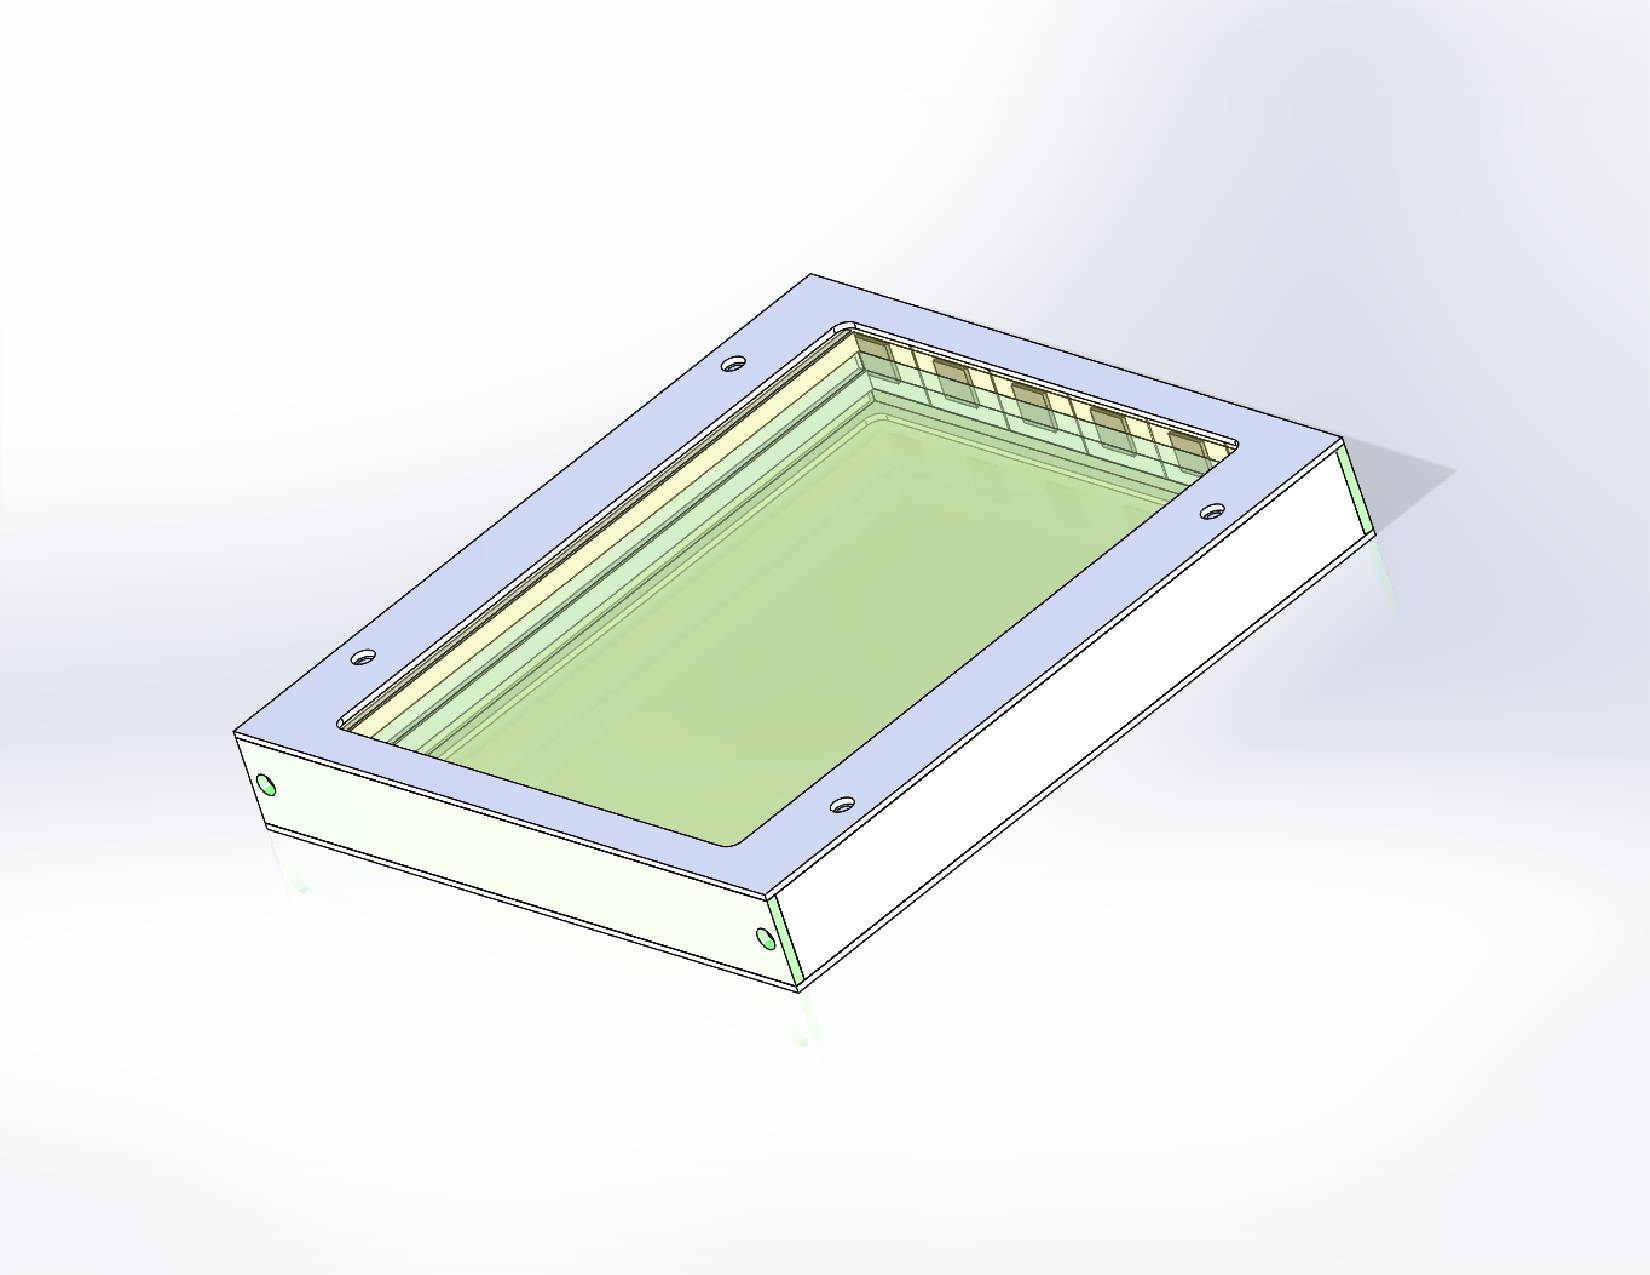
\includegraphics[height=.25\textheight]{pds-x-arapuca-cell}
  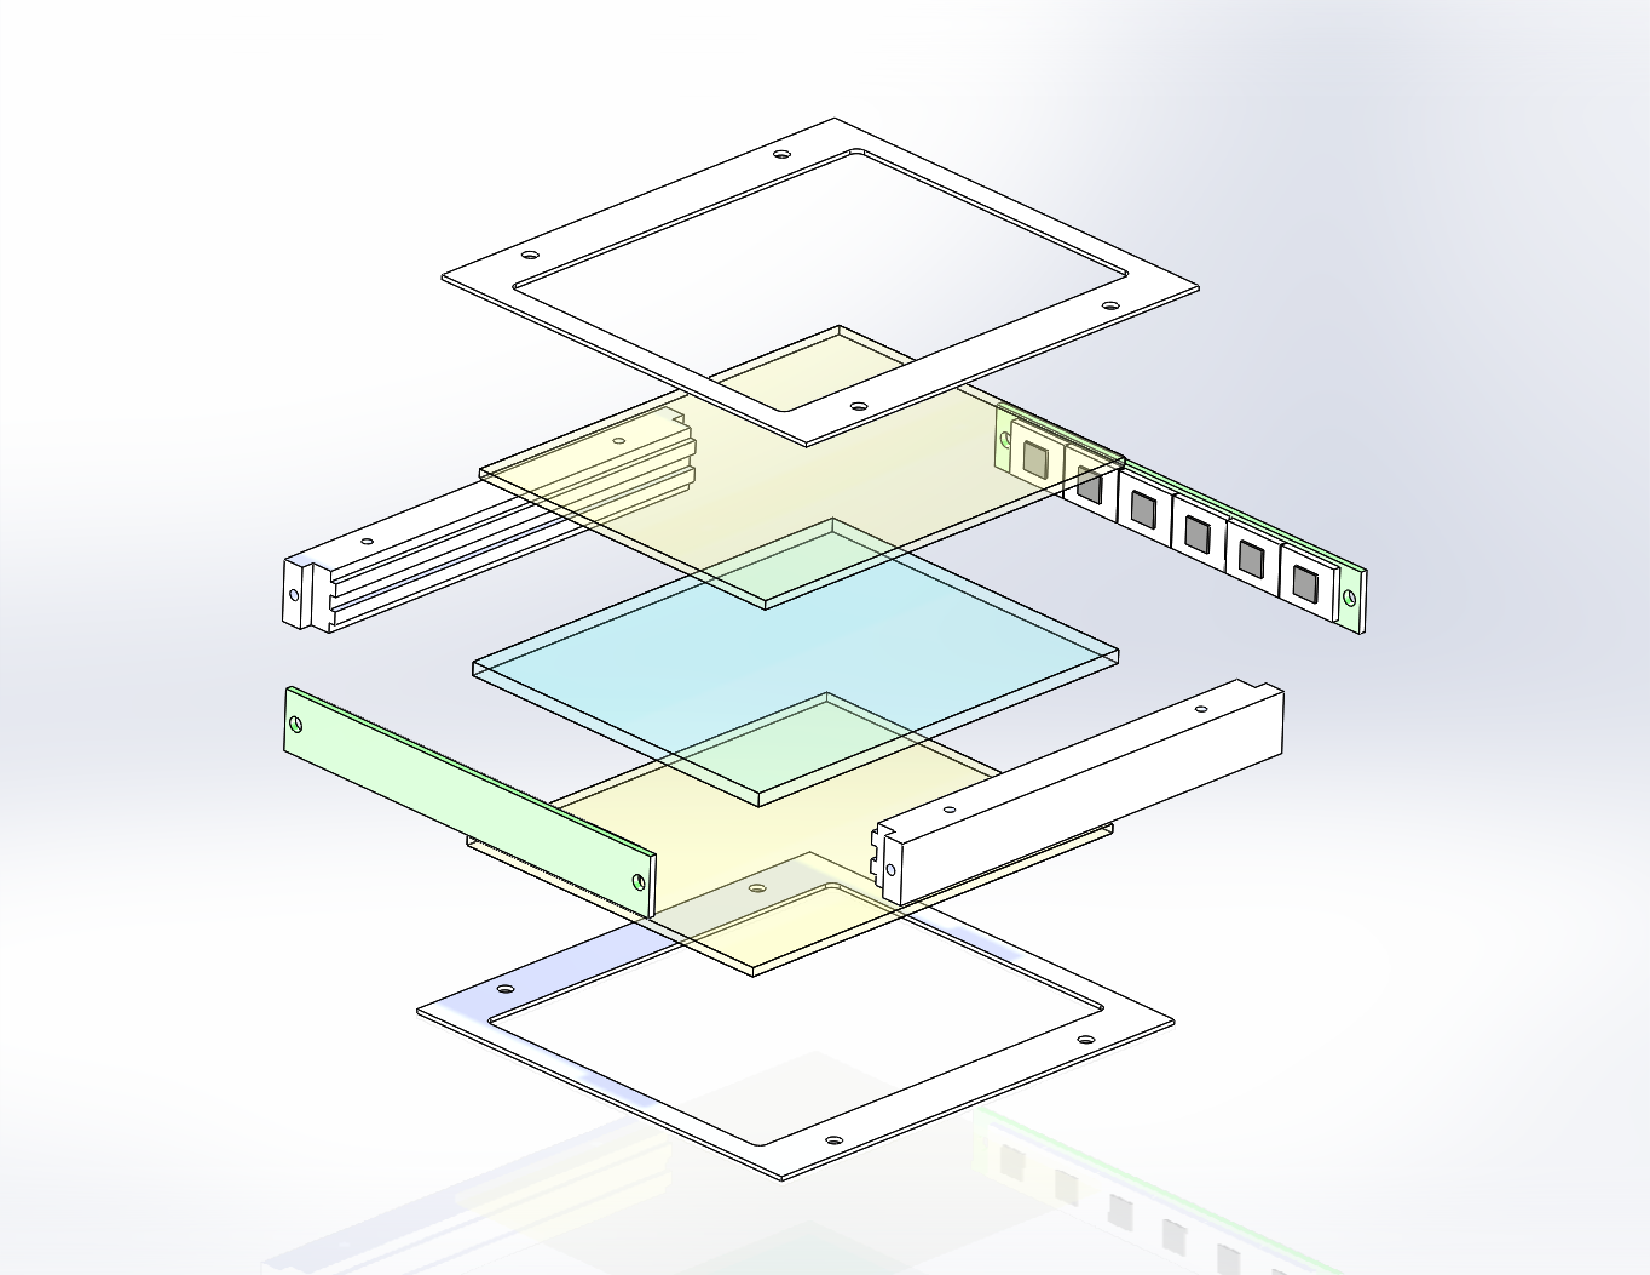
\includegraphics[height=.25\textheight]{pds-x-arapuca-exploded-view}
\end{dunefigure}

%\fixme{modifying descriptive text below}
%In the \dword{xarapu} design, Figure~\ref{fig:pds-x-arapuca-cell}, the inner shifter coating/lining over the reflective walls of the box is replaced by a thin wavelength-shifting light guide slab inside the box, of the same dimensions of the acceptance filter window and parallel to it. The \dword{sipm} arrays are installed vertically on the sides of the box, parallel to the light guide thin ends. 
%In the \dword{xarapu} design, Figure~\ref{fig:pds-x-arapuca-cell}, a single acrylic wavelength shifting light guide (Eljen EJ-296) 
The light guide inside the cell is positioned behind an array of six dichroic filters and parallel to them. 
% \fixme{Anne proposes to remove: This thin wavelength-shifting slab replaces the inner shifter coating over the reflective walls in the \dword{pdsp} \dword{sarapu} design. }
This design is easily configurable to detect light from just one side, as required for the side \dword{apa}s, or from both sides for the central \dword{apa}s. 

For dual-sided \dword{xarapu} modules, dichroic filters are placed on both sides of the %WLS bar. 
cell facing the \lar volumes.  In the case of the single-sided device, the back side of the cell  %dichroic filter is replaced by 
has a layer of highly reflective Vikuiti\footnote{3M Vikuiti\texttrademark\  ESR - http://multimedia.3m.com/mws/media/193294O/vikuiti-tm-esr-application-guidelines.pdf} to act as %the rear
a  reflector.  In both cases, the \dword{sipm} arrays are installed on two of the narrow sides of the cell perpendicular to the windows, parallel to and up against the light guide thin ends. Half of the \dword{sipm} active detection area collects photons from the light guide, a quarter of the area on either side of the guide is free to collect the fraction of photons reflected off the cell walls and windows. 
%\{check -Anne added this} - amended rjw

The basic mechanical design of the \dword{xarapu}-based \dword{pd} modules  
is similar to that of the two prototypes produced for \dword{pdsp}. Modifications to the prototype design include:  mechanical changes to allow for single-sided or dual-sided readout; increase in light collection area made possible by larger slots in the \dword{apa}; and modifications to the cabling and connector plan required to move the \dword{pd} cables out of the \dword{apa} side tubes, while reducing the cable requirements to one cat-6 cable per \dword{pd} module.

%\fixme{can we remove this sentence? Here we describe the design, fabrication and assembly envisaged based on that experience and these evolved design considerations. (anne)}

An \dword{xarapu} module is shaped like a bar with external dimensions of \SI{209.2}{cm} $\times$ \SI{11.8}{cm} $\times$ \SI{2.3}{cm},  allowing insertion between the wire planes through each of the ten slots in an \dword{apa}. 

%{figure of full PD module (with outside dimensions) here}

\begin{dunefigure}[A full \dword{xarapu} module overview]
{fig:pds-x-arapuca-full-module}
{A full \dword{xarapu} module overview. A module, which spans the width of an \dword{apa}, includes 24
 \dword{xarapu} cells, grouped into a set of four supercells of six cells each. In the center, active ganging PCBs collect the signals and mechanically join the supercells.}
% tweaked rjw \{check anne's update to figure caption~\ref{fig:pds-x-arapuca-full-module}}
 %two-sided x-arapuca 4/14/18
   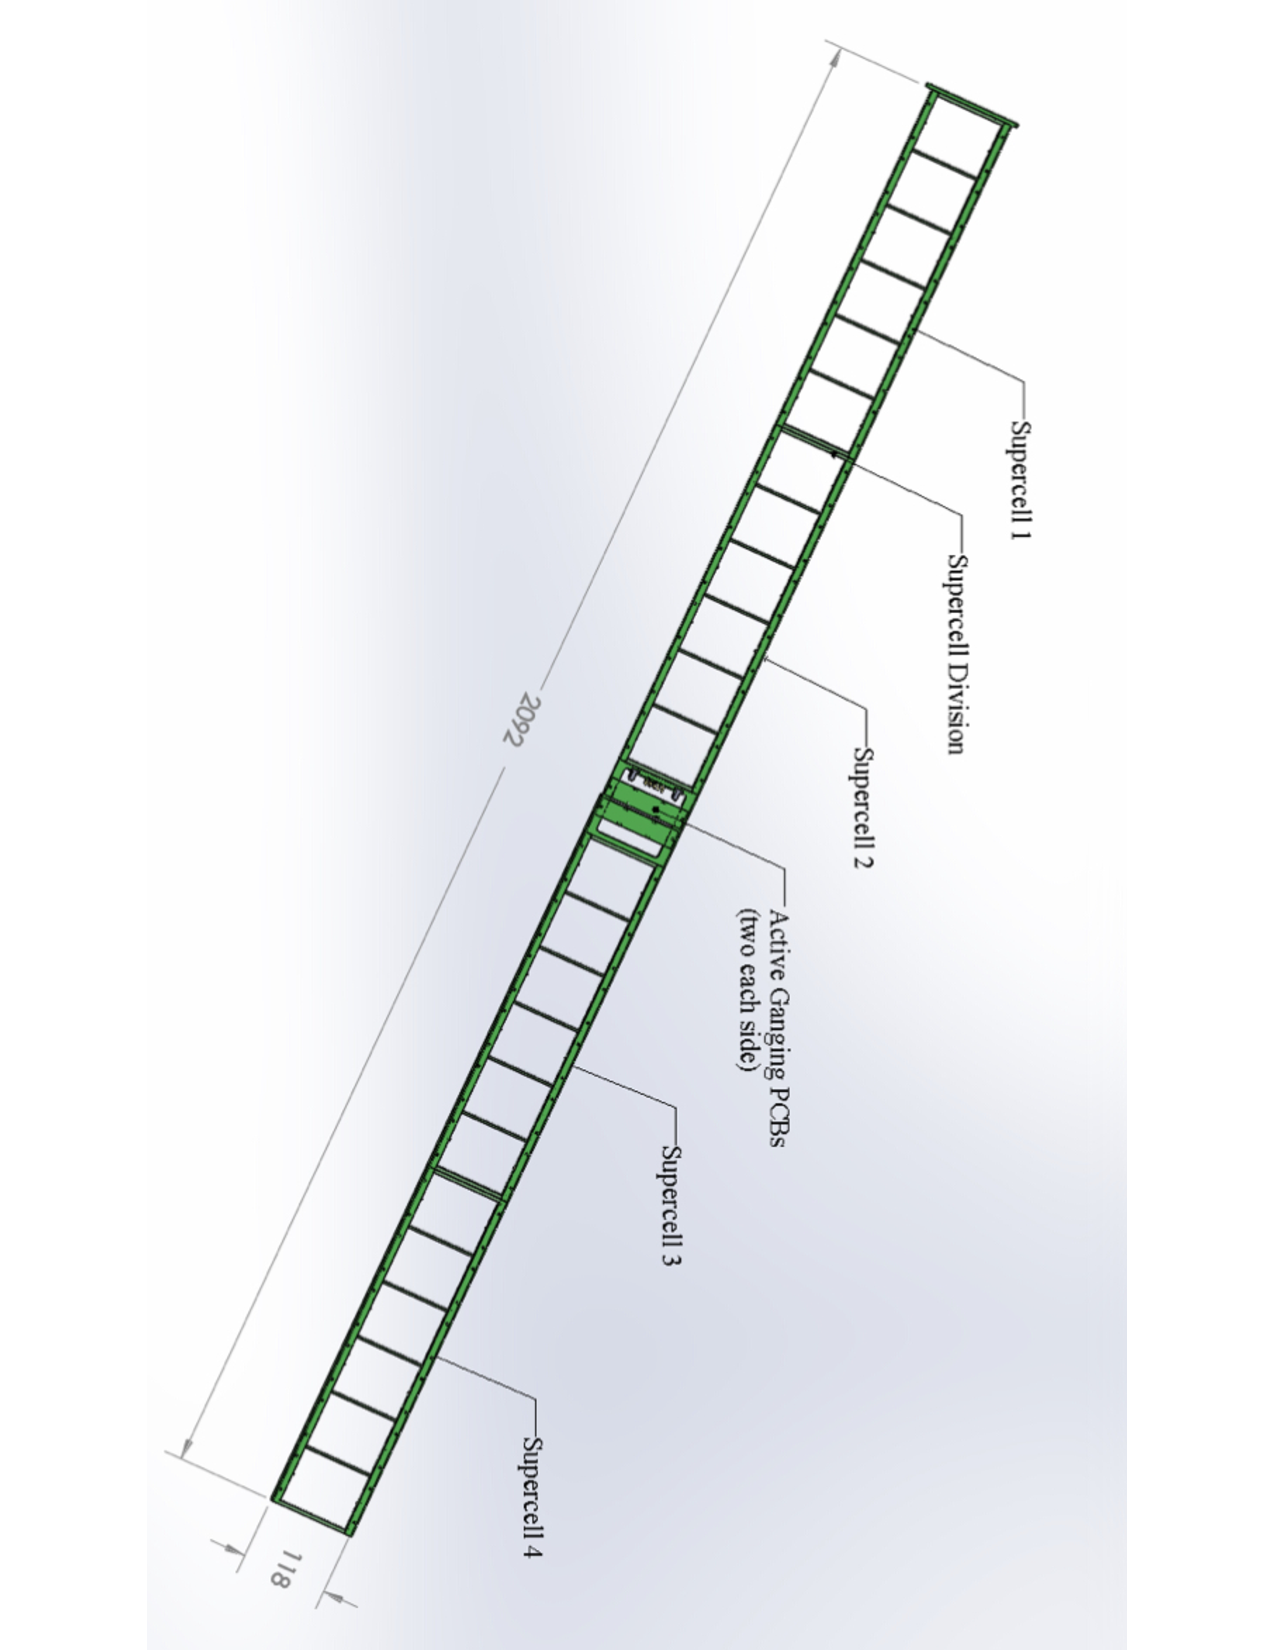
\includegraphics[angle=90,width=17cm]{pds-design-full-module-dimensioned}
  %\vspace{-2.5cm} 
\end{dunefigure}

The module contains four \dword{xarapu} supercells, each with six dichroic filter-based optical windows (for the single-sided readout) or 12 windows (double-sided readout) with an area of \SI{7.8}{cm} $\times$ \SI{9.3}{cm}.  The internal dimensions of  a supercell are approximately \SI{48.8}{cm} $\times$ \SI{10.0}{cm} $\times$ \SI{0.8}{cm}. A \dword{wls} plate (Eljen EJ-286) of dimensions \SI{48.7}{cm} $\times$ \SI{93.0}{cm}$\times$ \SI{0.35}{cm} is centered in the supercell midway between the dichroic windows.  

\begin{dunefigure}[Exploded \dword{xarapu} supercell.]{fig:pds-x-arapuca-exploded-Detail}
{Detailed exploded view of \dword{xarapu} supercell. Note that components are designed to be cut from FR-4 G-10 sheets to simplify fabrication.}
 % \vspace{-2.5cm}
 %two-sided x-arapuca 4/14/18
   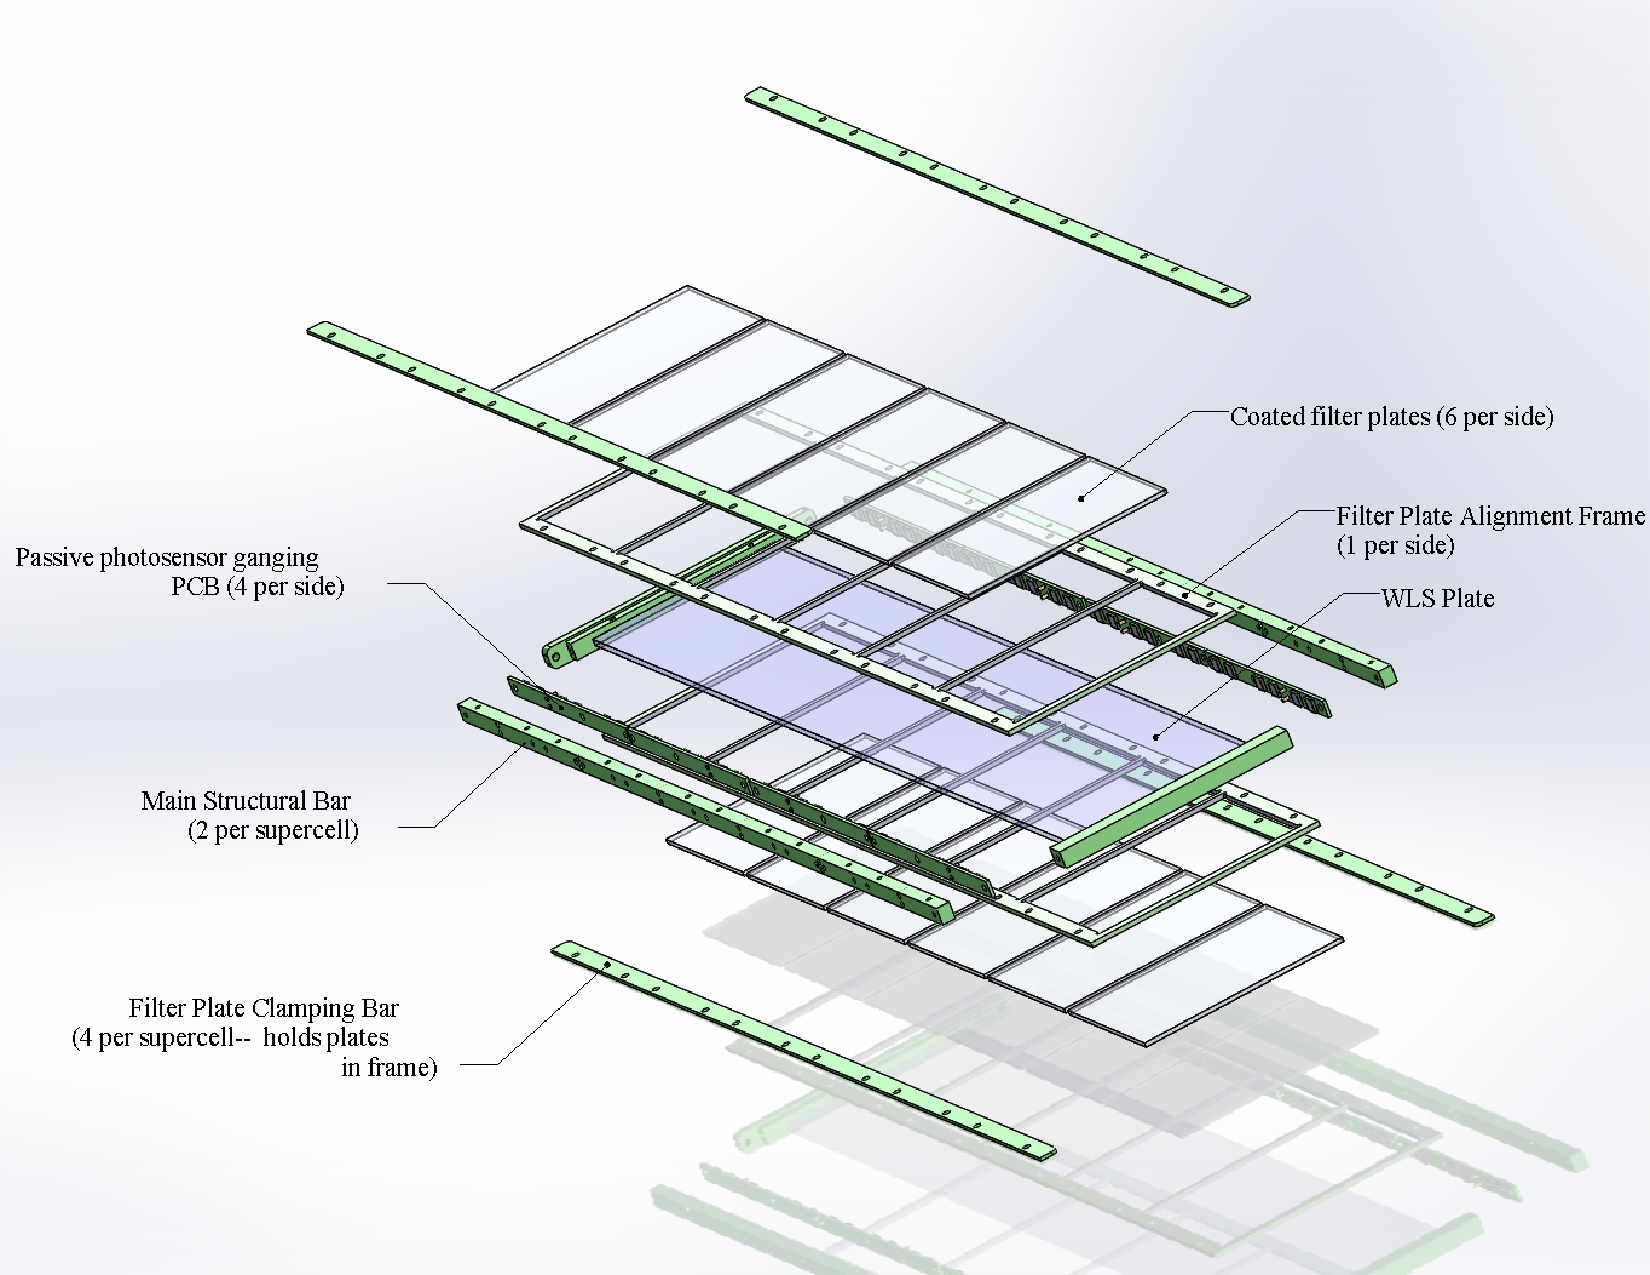
\includegraphics[height=.5\textheight]{pds-exploded-supercell-assembly-r2}
 % 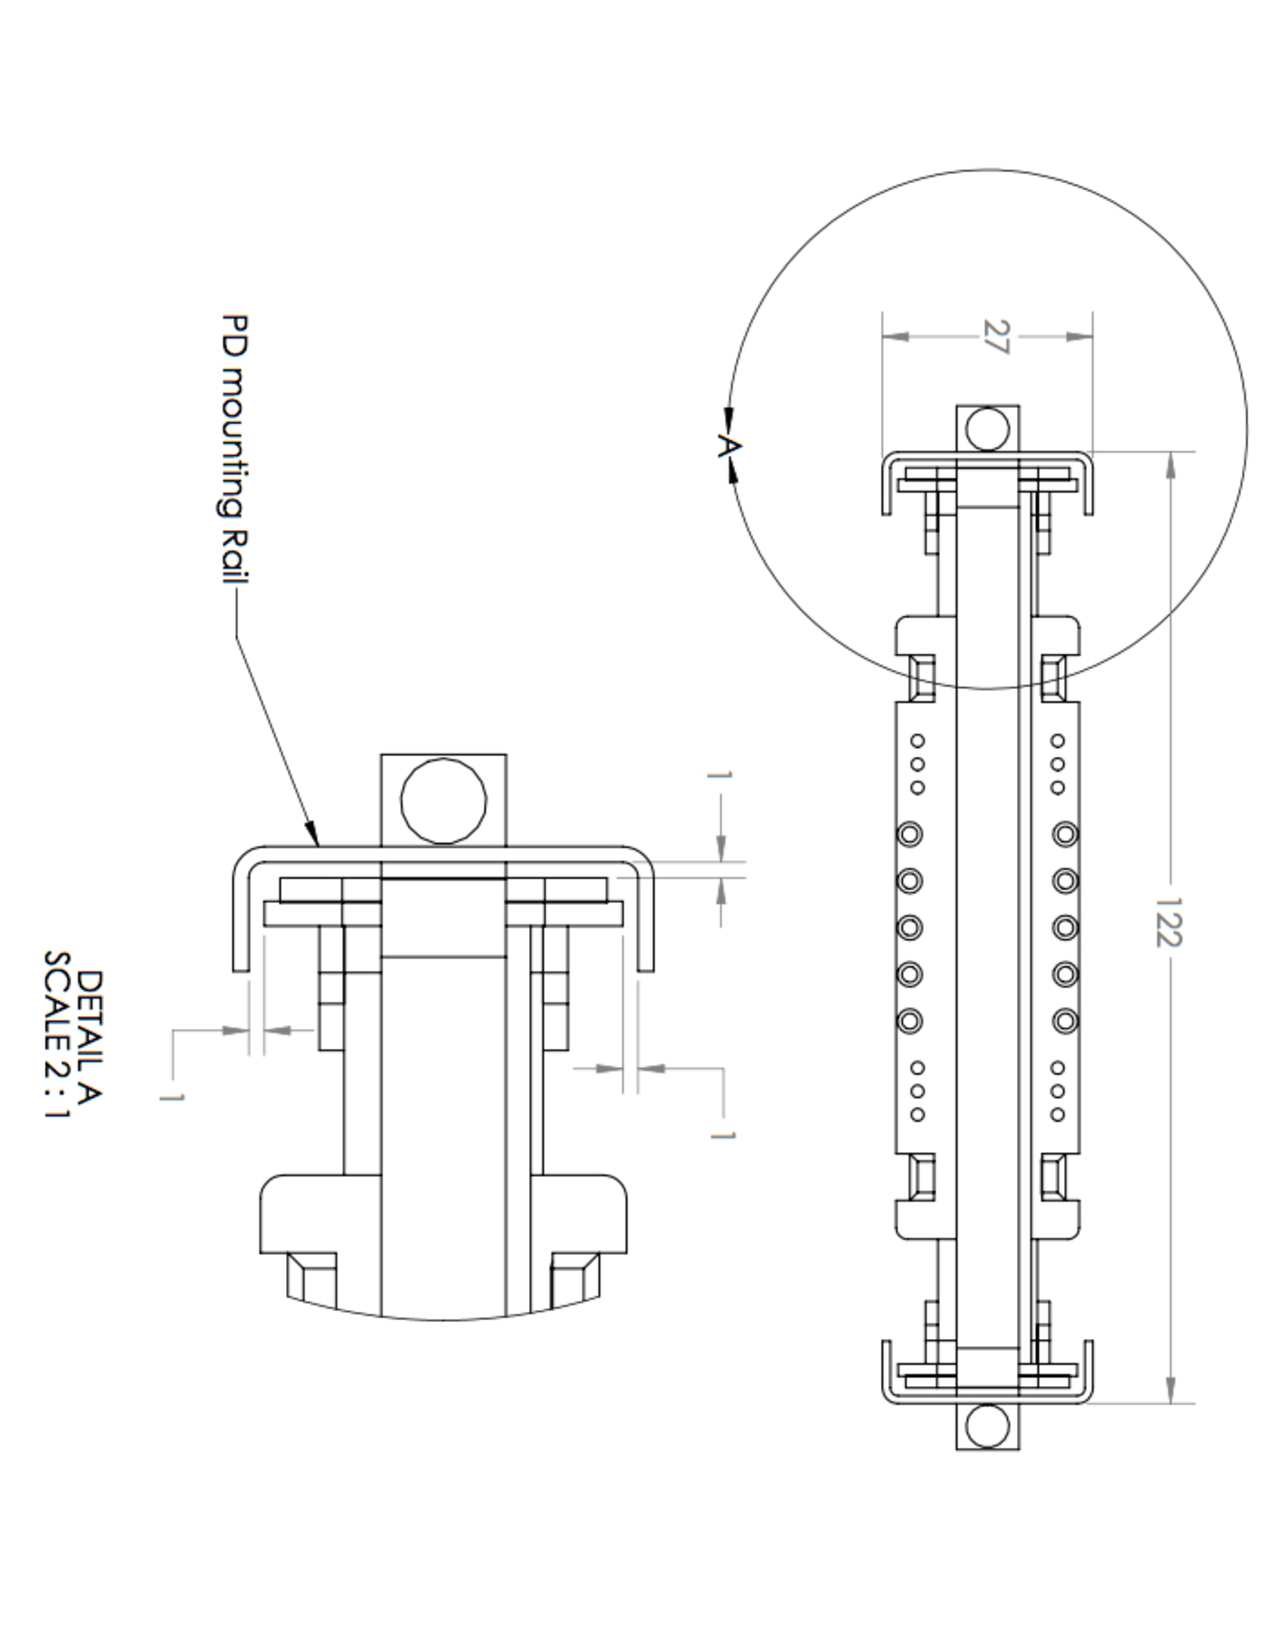
\includegraphics[height=.25\textheight]{pds_design_dimensioned_cross_section}
\end{dunefigure}

To reduce production costs and simplify fabrication, most of the \dword{pd} components are designed to be water-jet cut from sheets of FR-4 G-10 material, with minimal post-cutting machining required (mostly the tapping of pre-cut holes).  The current design contains many small fasteners; we will investigate replacing some of the fasteners with epoxy lamination of cut sheets where appropriate and cost effective, as the design process matures.

The \dwords{sipm} are mounted to PCBs positioned on the long sides of the supercell.  
The \dwords{sipm} are passively ganged in groups of six to photosensor mounting boards.

 Before mounting into the \dword{xarapu} module the boards are tested at room and LN2 temperatures. It is anticipated that production of the boards for the \dwords{spmod} will be done outside the USA, and South American institutions will optimize the design.
 %\{latin am or south - pick one} 
 Each supercell uses eight %mounting boards are used per supercell 
 to accommodate the 48 \dwords{sipm}.  The ganged signal outputs from these boards are connected to traces in signal routing boards at the edge of the \dword{pd} module. These signal routing boards also act as mechanical elements in the design, mechanically joining the supercells and providing for rigidity.  These PCBs are four-layer boards, approximately \SI{104.6}{cm} $\times$ \SI{2.3}{cm} $\times$ \SI{0.15}{cm}.

 \begin{dunefigure}[\dword{xarapu} SiPM mounting and signal routing boards.]
 {fig:mounting-board-routing-board}
{Model of photosensor mounting board (left) and signal routing PCB (right) for \dword{xarapu} module.  Six Hamamatsu \dwords{mppc} are passively ganged and the ganged signals transmitted along the routing board to the active ganging circuits in the center of the module}
 % \vspace{-2.5cm}
  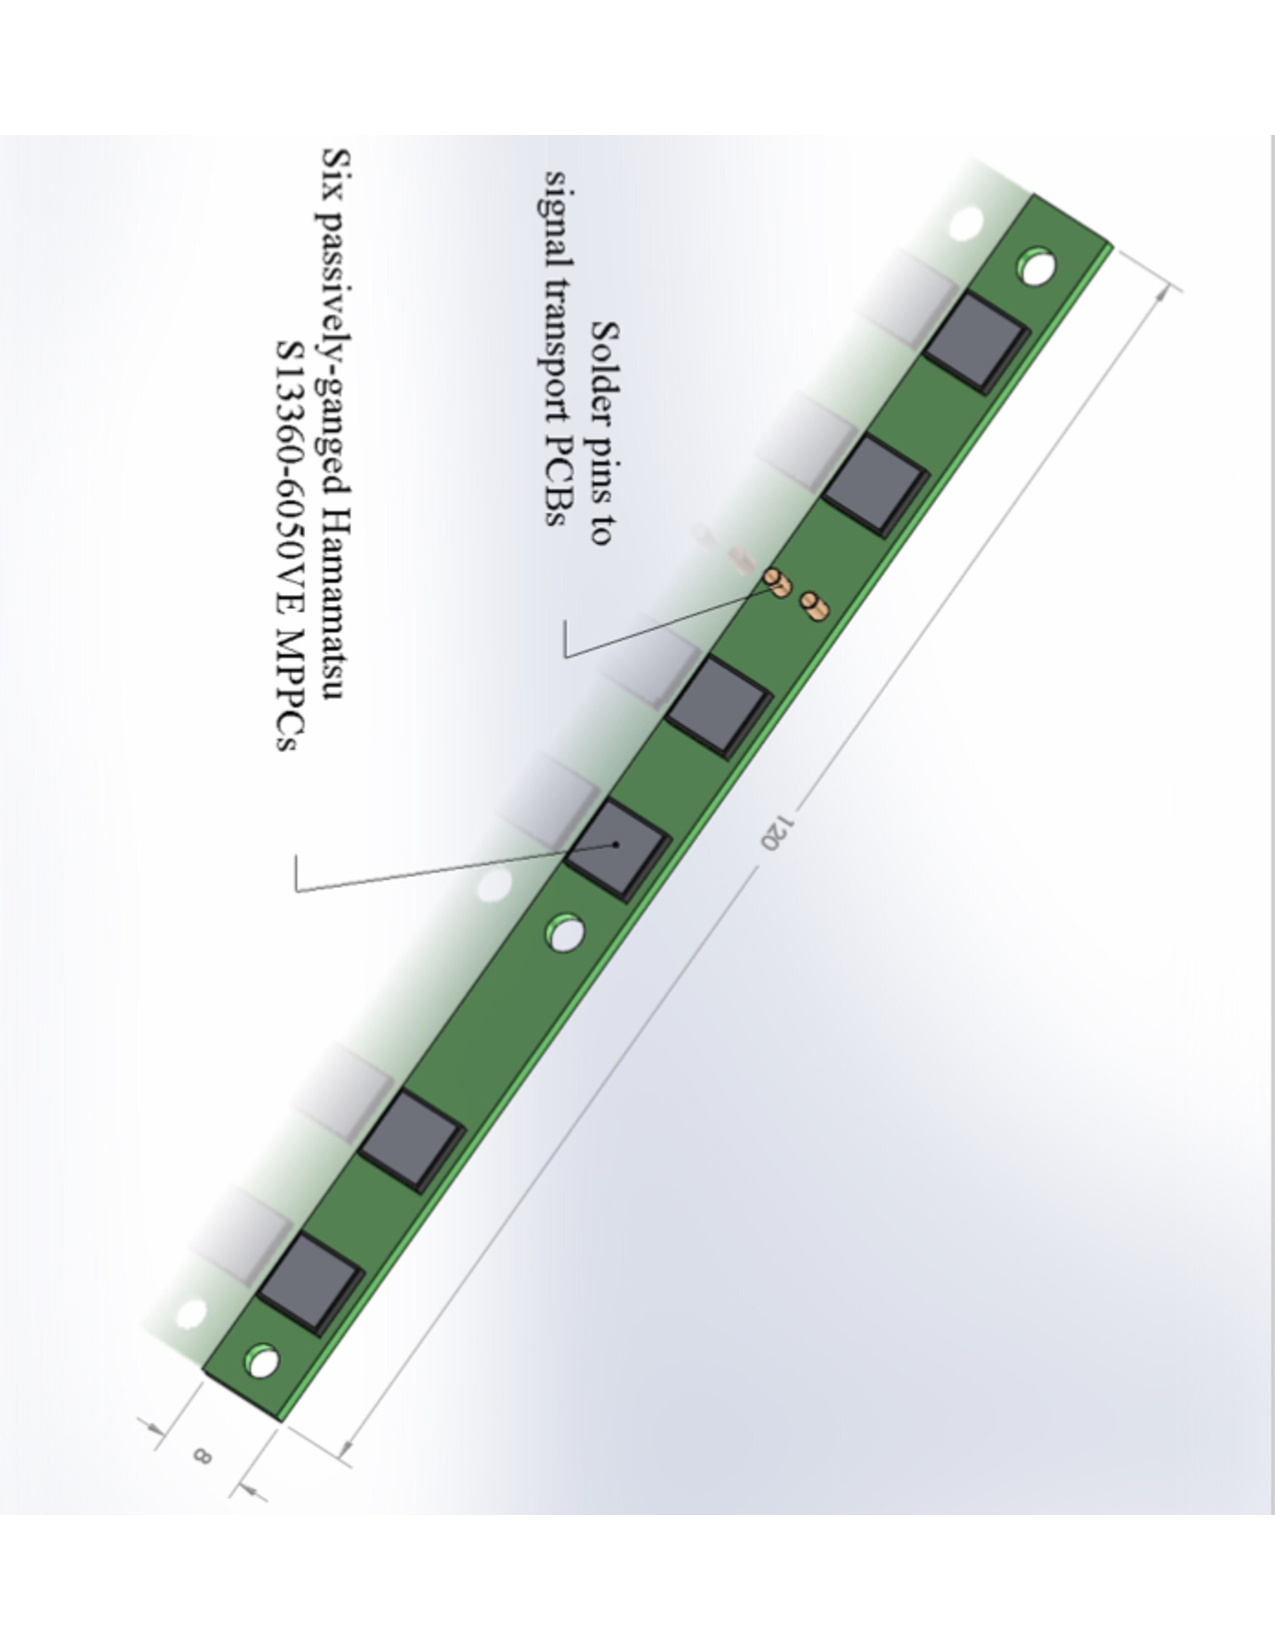
\includegraphics[angle=90,height=6cm]{pds-photosensor-mounting-board-r2}
  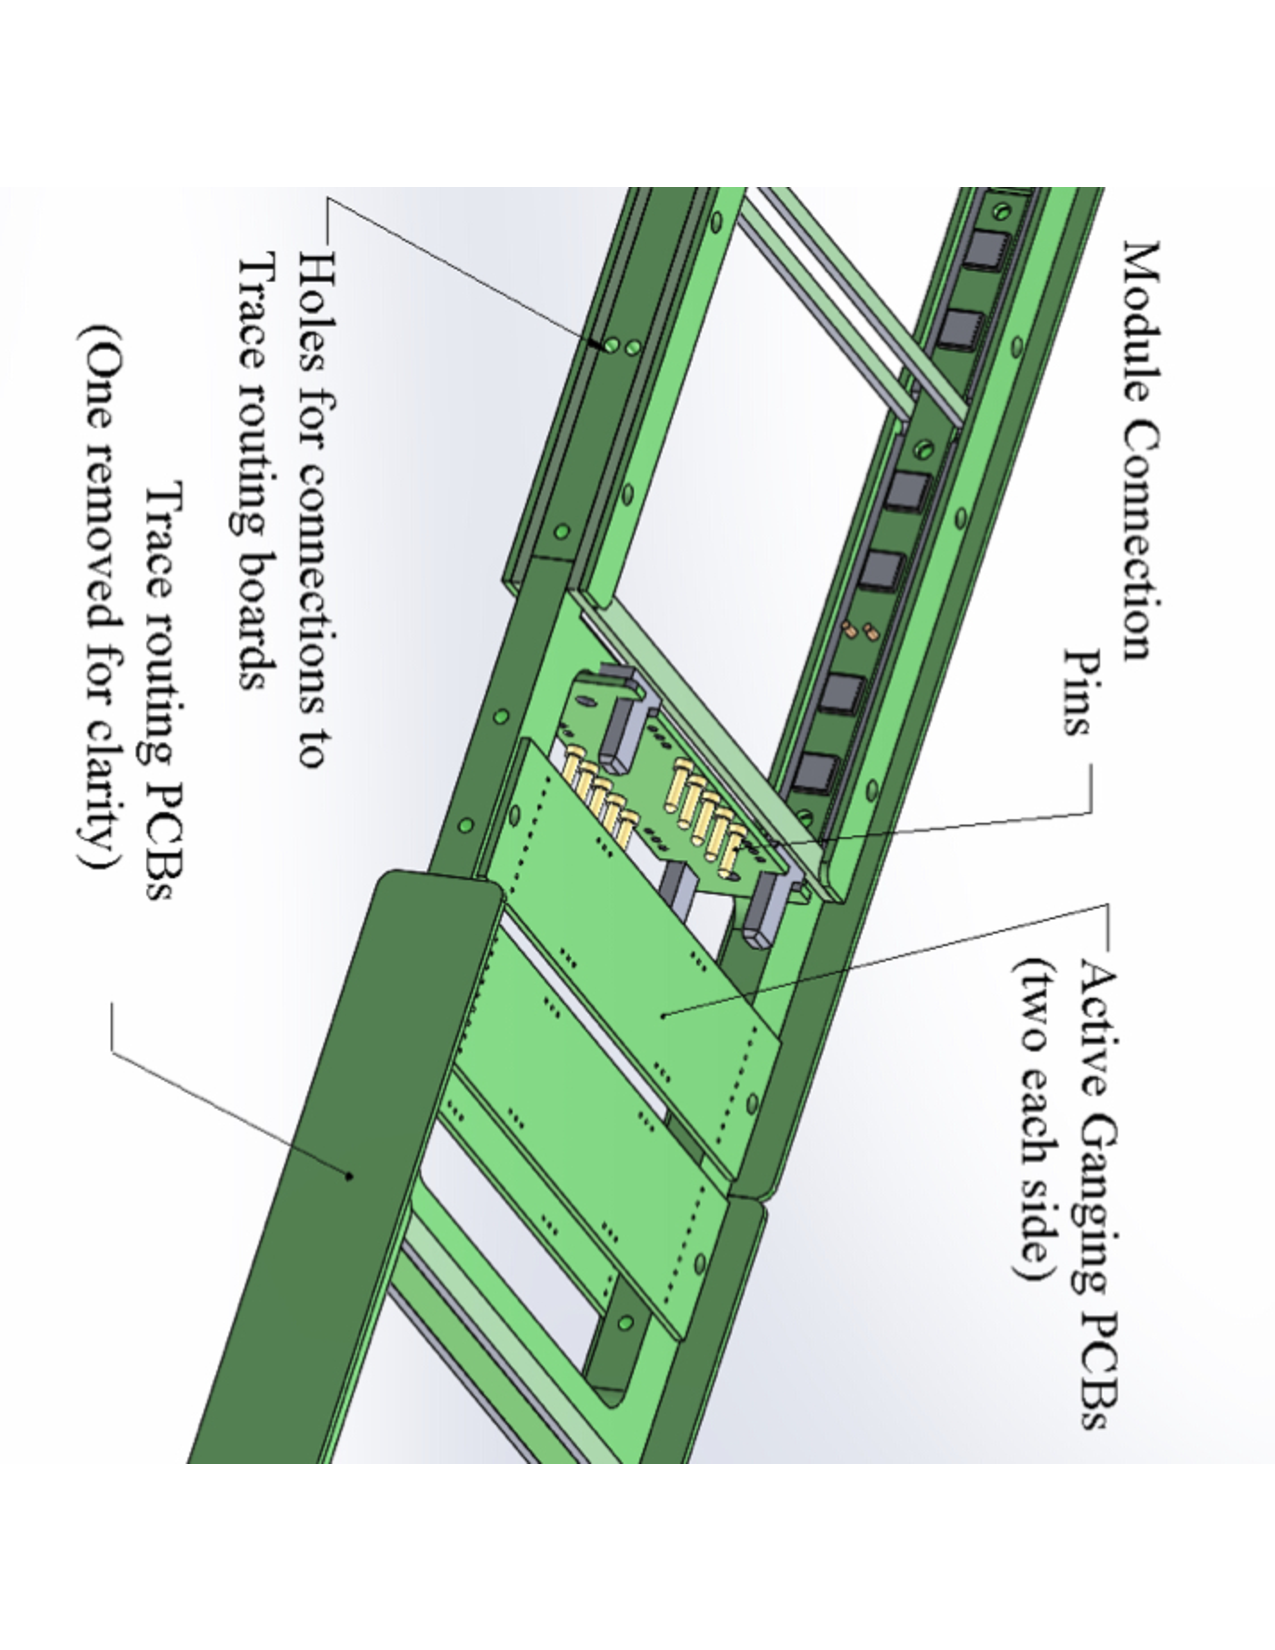
\includegraphics[angle=90,height=6cm]{pds-trace-routing-pcb}
\end{dunefigure}
The passively ganged signals are then routed through these boards to an active-ganging PCB at the center of the module, where all eight passively ganged signals from a single supercell are actively ganged into one output channel. This summed output from a single supercell is then connected to a single twisted pair in the cat-6 readout cable for the module.  The active ganging PCBs (one per supercell, four per module) are positioned in the module so that they are located inside the central \dword{apa} mechanical support tube when fully installed.

%\{?? add pictures of module center showing active ganging PCBs outside \dword{apa}, and buried in central tube} leave out for now

%remove the of standard arapucas used for protodune
%\begin{dunefigure}[\dword{pdsp} ARAPUCA modules during assembly.]{fig:arap-prod01}
%{\dword{pdsp} ARAPUCA modules during assembly prior to installation of the dichroic filters; \dwords{sipm} and TPB coated reflector are visible.}
%  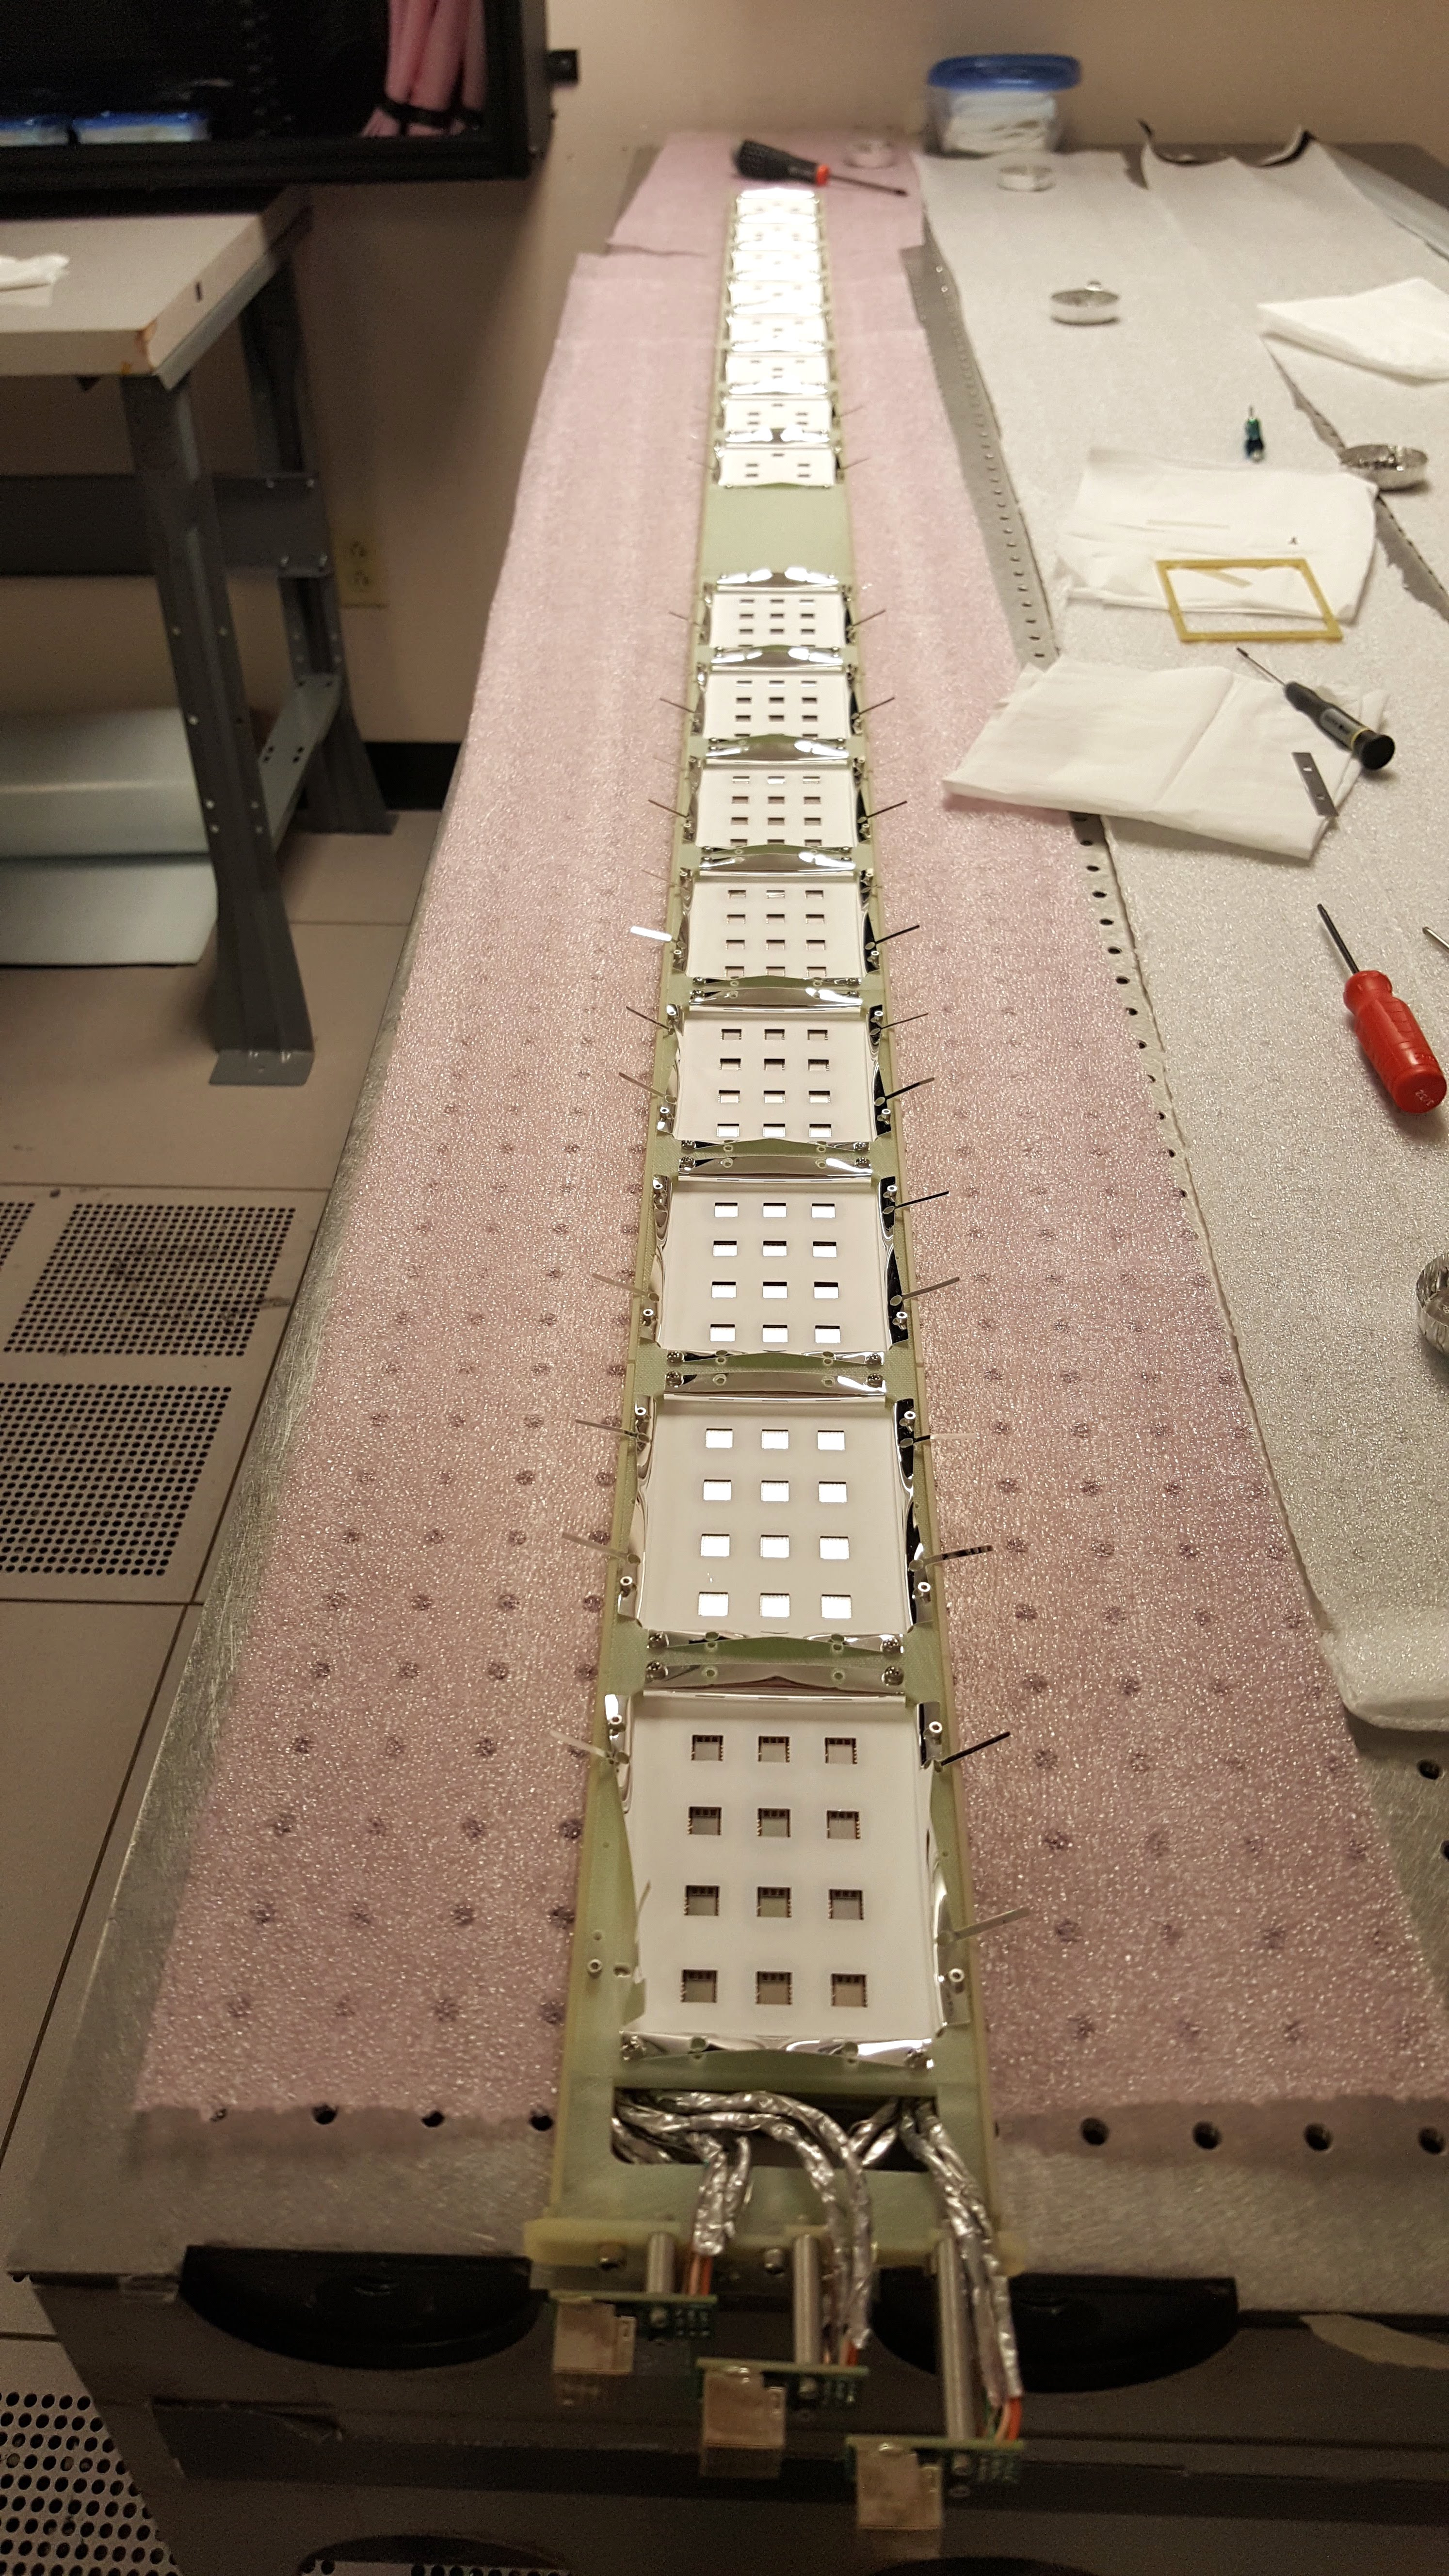
\includegraphics[height=8cm]{pds-arapuca-protodune02-apr18}
%\end{dunefigure}

The  internal surface of the sides the cell are lined with an adhesive-backed dielectric mirror foil laser cut with openings at the locations of the \dwords{sipm}.  In the case of the single-sided readout the dichroic filter windows on the non-active side of the cell are replaced by a blank FR-4 G-10 sheet, lined in the cell interior with a Vikuiti reflector foil. %these are visible in Figure~\ref{fig:arap-prod01}, which shows an ARAPUCA during assembly prior to installation of the optical windows.

%The backplane \dword{sipm} boards for the \dword{pdsp} modules were designed at CSU and produced by an external USA vendor\footnote{Advanced Circuits Inc.; www.4pcb.com.}; the \dwords{sipm} were soldered on the boards using a reflow oven at CSU. Before mounting into the ARAPUCA module they were tested at room and LN2 temperatures. It is anticipated that the production of the boards for  \dwords{spmod} will be done outside the USA. %move to Brazil.
 %and the design will be optimized by South American institutions in collaboration with CSU.
%\{want to specify Brazil?} - leave as SA

The optical window(s) of each supercell are dichroic filters with cut-off at \SI{400}{nm}. While the filters used for the \dword{pdsp} prototypes have been acquired from Omega Optical Inc.\footnote{http://www.omegafilters.com/}, other vendors are being considered for the DUNE production\footnote{ASHAI -Japan, Andover-USA, Edmunds Optics-USA}.
% rjw 12/2/18 the following moved to Prod and Assembly
%Prior to coating, the filters are cleaned according to the procedures given by the manufacturer using isopropyl alcohol. Since the most likely vector for scratching/damaging the coating is dragging contaminated wipes across the surface, new clean lint free wipes are used for each  cleaning pass on the surface. Clean filters are then baked at 100$^\circ$C for \SI{12}{hours}.    
   
The filters are coated on the external side facing the \lar active volume with pTP\footnote{p-TerPhenyl, supplier: Sigma-Aldrich\textregistered.}.  The coatings for the \dword{pdsp} modules have been made at the thin film facility at \fnal using a vacuum evaporator. Each coated filter was dipped in LN2 to check the stability of the evaporated coating at cryogenic temperature. 


\section{Silicon Photosensors}
\label{sec:fdsp-pd-ps}
%\metainfo{\color{blue} Content update: Zutshi}

\fixme{rjw 1/13/19 The following moved from what was originally a design considerations section...but converted by Anne to an overview, so this was too much detail. Moved the summary that was here in the Design section to there. Need to condense to a shorter narrative and get to the bottom line.} 

%%%%%%%%%%%%%%%%%%%%%%%%%%%%%%%%%%%%%%%%%%%%%%%%%%%%%%%%%%%
%rjw 12/1/18 the following moved from the Design section
The following summarizes the most salient guiding principles and requirements for this \dword{sipm}-based photodetection system.

\begin{itemize}
\item  The physics goals and the photon collection implementation determine the full suite of \dword{sipm} %requirements 
specifications (e.g., number of devices, spectral sensitivity, dynamic range, triggering, zero-suppression threshold).  As discussed in Section~\ref{sec:fdsp-pd-intro},  the requirements for \dword{snb} neutrinos are not yet fully established, however R\&D carried out to date indicates that  
performance characteristics of devices from several vendors are close to meeting the %that needed for the 
\dword{pds} needs (see Table~\ref{tab:photosensors}). 
Nearly one thousand of several types of these devices are used in the \dword{pdsp} \dword{pd}\footnote{\dword{pdsp} \dword{pds} uses 516 sensL MicroFC-60035C-SMT, 288 Hamamatsu MPPC 13360-6050CQ-SMD with cryogenic packaging, 180 Hamamatsu MPPC 13360-6050VE.},  %, which will 
providing an excellent test bed for evaluation and monitoring of \dword{sipm} performance in a realistic environment over a period of months. Results from this are summarized in Section~\ref{sec:fdsp-pd-validation}.

\item A key requirement is to ensure the mechanical and electrical integrity of these devices in a cryogenic environment. %However, 
Currently, catalog devices for most vendors are certified for operation only down to \num{-40}$^\circ$C. It is essential to be in close communication with  vendors in the %design, fabrication and \dword{sipm} packaging certification stages 
\dword{sipm} design, fabrication and packaging certification stages to ensure %that the device will be robust and reliable for long-term operation in a cryogenic environment. 
robust and reliable long-term operation in a cryogenic environment. 
Two %sources 
vendors have expressed interest to engage with the consortium in this fashion
with the goal of %having the vendor warranty 
providing a warranty of the product for our application: Hamamatsu Photonics K.K., a large well-known commercial vendor in Japan and Fondazione Bruno Kessler (FBK) in Italy. FBK is an experienced developer of solid state photosensors that typically licenses its technology;  it is partnering with the DarkSide collaboration to develop devices with specifications very similar %requirements as DUNE.
to DUNE's. 
%Contact with other vendors and experiments using this technology in a similar environment is also being pursued. 

\item DUNE needs to carry out comparative performance evaluation of promising \dword{sipm} candidates from
multiple vendors %will need to be carried out 
in parallel over the next year. This evaluation will %need to
address inherent device characteristics (e.g., gain, dark rate, x-talk, after-pulsing) that are common to all three %photon collector 
options, along with ganging performance, form factor, spectral response, and mechanical mounting options that may have different optimizations for the two light guide designs and ARAPUCA.
Experience acquired from \dword{pdsp} construction and operation will inform QA/QC plans for the full detector.


\item Size constraints and other considerations imply that the signal output of \dwords{sipm} must be electrically ganged.  The area of current candidate \dwords{sipm} is less than \SI{1}{cm$^2$}, providing a much finer granularity than needed. In addition, the cold feedthrough size and space in the \dword{apa}s for cable runs limits the number of \dword{pd} signal and power cables. 
The degree of ganging depends on the number of individual \dwords{sipm} needed to achieve the required light yield. For the \dword{xarapu} this is expected to be in the range of \num{12} to \num{48} \dwords{sipm} per channel. 
Simple passive-ganging (wiring the outputs together) and active-ganging (with active components) have been investigated.

\item The terminal capacitance of the sensors strongly affects the \dword{s/n} when devices are ganged in parallel and thus is a factor in \dword{sipm} selection. It may ultimately determine the maximum number of individual sensors that can be ganged this way. 
\end{itemize}

%%%%%%%%%%%%%%%%%%%%%%%%%%%%%%%%%%%%%%%%%%%%%%%%%%%%%%%%%%%


% rjw 12/1/18 Moved from the overview section
As noted previously, we have selected a \SI{6}{mm}$\times$\SI{6}{mm} \dwords{mppc}  
produced by Hamamatsu as the current baseline \dword{sipm} device.  
We are also vigorously pursuing an alternative based on the design of a device developed for operation in \lar by the DarkSide experiment collaboration and FBK.

The baseline \dword{pds} design has 192 \num{6}$\times$\SI{6}{mm$^2$} \dwords{mppc} per \dword{pd} module with groups of 48 \dwords{mppc} electrically ganged into four electronics readout channels. This leads to a total of 288,000 \dwords{mppc} per \dword{spmod}. The ganging (signal-summing) scheme is described in the next section.


%As implemented in \dword{pdsp}, there are twelve \num{6}$\times$\SI{6}{mm$^2$} \dwords{sipm} per bar and \numrange{6}{12} per ARAPUCA box.
%With this configuration, a \nominalmodsize \dword{spmod} with \num{150} \dwords{apa}, each with \num{10} \dword{pd} modules, would contain \num{18000}-\num{36000} (single or double-ended readout) \dwords{sipm} for the light guide designs and 10-20 times more for the higher granularity ARAPUCA design. This corresponds to approximately \num{1}-\SI{13}{m$^2$} of active \dword{sipm} surface area.

%{ rjw 11/25/18 reduced table to just Hamamatsu and up to two FBK device -- values to be inserted}
\begin{dunetable}[Candidate photosensors characteristics.]
{p{0.18\textwidth}p{0.18\textwidth}p{0.18\textwidth}p{0.18\textwidth}}
{tab:photosensors}
{Candidate Photosensors Characteristics.}
	                      &Hamamatsu (Baseline)   & Hamamatsu-2    & FBK                 \\ \toprowrule
Series part \#            & S13360                &     S14160         & NUV-HD-LF         \\ \colhline
Vbr (typical)                 & 50 V to 52 V          &   36 V to 38 V & 31 V to 33 V                \\ \colhline
Vop (typical)                 & Vbr + 3 V             &   Vbr + 2.5    & Vbr + 3 V                \\ \colhline
Temp. dependence          & 54 mV/K               &       35 mV/K      & 25 mV/K            \\ \colhline
Gain                      & $1.7 \times 10^6$     &      $2.5 \times 10^6$ &       $0.75 \times 10^6$          \\ \colhline
Pixel size                & 50 $\mu$m             &       50 $\mu$m    & 25 $\mu$m            \\ \colhline
Size                      & 6 mm x 6 mm           &     6 mm x 6 mm    & 4 mm x 4 mm            \\ \colhline
Wavelength                & 320 to 900 nm         &     280 to 900 nm  & 280 to 700 nm            \\ \colhline
PDE peak wavelength       & 450 nm                &        450 nm      & 410 nm            \\ \colhline
PDE @ peak                & 40\%                  &        50\%        & 50\%            \\ \colhline
DCR @ 0.5PE               & < \SI{50}{\kilo\hertz\per\square\milli\meter}      & < \SI{100}{\kilo\hertz\per\square\milli\meter}   & < \SI{25}{\kilo\hertz\per\square\milli\meter}               \\ \colhline
Crosstalk                 & <3\%				  &      <7\%          & <3\%             \\ \colhline
Afterpulsing              &                       &                &                 \\ \colhline
Terminal capacitance      & \SI{35}{\pico\farad\per\square\milli\meter}          &   \SI{55}{\pico\farad\per\square\milli\meter}     &      \SI{50}{\pico\farad\per\square\milli\meter}         \\ \colhline
Lab experience            & Mu2e and DUNE prototypes      &                &     Darkside  \\         
\end{dunetable}


%%%%ELECTRONICS %%%%%%%%%%%%%%%%%%%%%%%%%%%%%%%%%%%%%%%%%%%%%%%%%%%

\section{Electronics}
\label{sec:fdsp-pd-pde}
%\metainfo{\color{red}\bf  Content: Djurcic/Franchi/Moreno/Spitz/Toups}

\fixme{It would be helpful to have a simple figure that shows the signal path - from SiPM to ganging to frontend electronics to \dword{daq} indicating cable path lengths and location with respect to the \dwords{apa} and cryostat.}

The \dword{pds}'s electronic readout system must (1) collect and process electrical signals from \dword{sipm}s reading out the light collected by the \dwords{xarapu}, (2) provide an interface with the trigger and timing systems supporting data reduction and classification, and (3) transfer data to offline storage for physics analysis.

%As specified in Table~\ref{tab:spec:time-resolution}, the readout system must 
As specified in Table~\ref{tab:specs:SP-PDS}, the readout system must enable the $t_0$ measurement of non-beam events; this capability will also enhance beam physics by recording interaction time of events within 
beam spill to help separate against potential cosmic background interactions. A highly capable readout system was developed for use with \dword{pdsp} and prototype development 
%\{other prototypes?} -- no
as described in Section~\ref{sec:ssp-protodune-electronics}. However, a more cost-effective wave form digitization system developed for the Mu2e experiment has been identified and selected as the baseline choice. 


%Physics simulation studies are currently underway to determine if pulse-shape discrimination will be required, which would provide the capability to record both prompt and delayed components of scintillation light (characteristic times of \SI{6}{ns} and \SI{1.3}{$\mu$s}), the latter consisting mostly of single photoelectrons and thus place stringent requirements on \dword{s/n} performance. 
% *** 12/3/18 Per Josh S  - the mu2e system can do this so can use for this purpose. No need to reference the studies.

This section describes the scheme used to electrically gang the signals from 48 \dwords{sipm} and the baseline \dword{fe} electronics system.


%Selection of the ganging option will include passive or active solutions, where the active 
%circuitry may require cold components such as an amplifier in the \lar volume. Design options with active cold components will need 
%to address issues of power dissipation and potential risks of single-point failures of multi-channel devices inside the cryostat.
%In the case of passive ganging, analog signals are transmitted outside of the cryostat for processing and digitalization. 
%Successful demonstrations of passive ganging at \lar temperatures have been made for groups of four and twelve 6x6 mm Micro-FC-60035C-SMT C series, and groups of 2, 4, 8, and 12  Hamamatsu \dwords{mppc} (S13360-6050PE) at  \num{25}$^\circ$C, - \num{70}$^\circ$C and \SI{77}{K}. 
%Active ganging has been demonstrated for an array of 12 sensL \num{4}$\times$\num{4} arrays of \SI{3}{mm}$\times$\SI{3}{mm} sensL C-series \dwords{sipm} (48 in all) and  72 \dwords{sipm} mounted in a hybrid combination of passive and active ganging using \SI{6}{mm}$\times$\SI{6}{mm} \dwords{mppc} with a low noise operational amplifier--this design combines 12 active branches into the op-amp, where each branch has six \dwords{mppc} in a parallel passive-ganging configuration.

\subsection{SiPM Signal Ganging}
\label{sec:pds-design-ganging}
%{Zelimir added this subsection}

Light collector techniques require electrical summing (ganging) of the \dwords{sipm} in order to maximize the active area of the photosensors while keeping the channel count reasonably low. The ganging of electrical signals from \dword{sipm} arrays is implemented to minimize the electronics channel count while maintaining adequate redundancy and granularity, as well as to improve the readout system performance.  
Technical factors that affect performance of the ganging system are the characteristic capacitance of the \dword{sipm} and the number of \dwords{sipm} connected together, which together dictate the \dword{s/n} and affect the system performance and design considerations.

We have demonstrated a feasible passive summing scheme with twelve Hamamatsu \dword{mppc} sensors now operational in \dword{pdsp}. For optimal performance in DUNE, we have shown that an ensemble of 48 Hamamatsu \SI{6}{mm}$\times$\SI{6}{mm} \dwords{mppc} can be summed into a single channel by a combination of passive and active ganging (see Section~\ref{sec:pds-valid-ganging}).  In this scheme, an amplifier is used to adjust the \dword{mppc} output signal level to the input of an \dword{adc}; the active summing is realized with an OpAmp THS4131. This combination of passive and active ganging with cold signal summing and amplification is the baseline for the \dword{pds}.

\fixme{Need a figure with the circuit showing the DUNE 6 passive x 8 active configuration}

In addition to the baseline scheme, a parallel effort is underway to investigate further optimization including development of detailed simulation and testing of prototype boards in South America. One scheme being investigated simulates the signals of 12 passively ganged \dwords{sipm} passed through a charge integrator or a charge amplifier transimpedance model into a summing stage. The simulation flow and the simulated response are shown in 
%Figure~\ref{fig:fig-pds-gang-jorge-1}(left) shows design scheme used in the simulation flow presented in 
Figure~\ref{fig:fig-pds-gang-jorge-1}. Figure~\ref{fig:fig-pds-gang-jorge-2} shows the circuit designed based on these studies to be used with the \dword{pd} in the \fnal ICEBERG test stand (Section~\ref{sec:iceberg-teststand}).

\begin{dunefigure}[Active summing board design simulation flow.]
 {fig:fig-pds-gang-jorge-1}
 {Active summing board design simulation flow (left) and simulated response of the circuit with 48 \dwords{sipm}(right).}
% {The active summing board design scheme (left) used in the simulation flow (right).}
%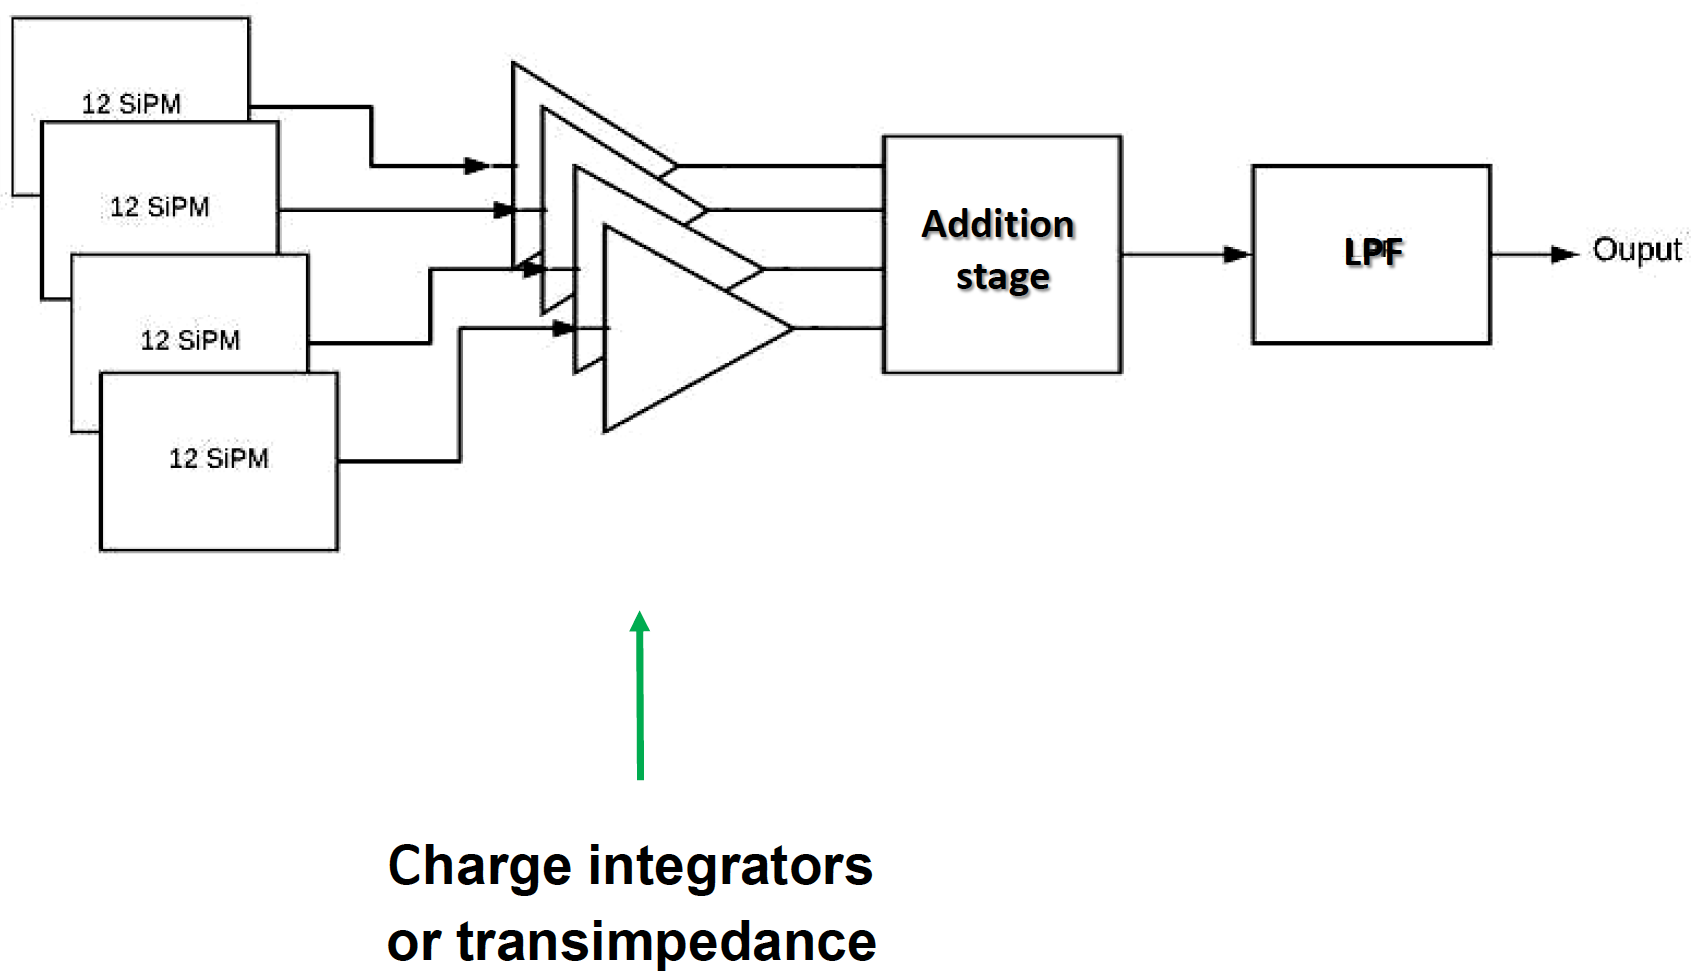
\includegraphics[angle=0,width=8.4cm,height=6cm]{graphics/pds-gang-jorge-1.png}
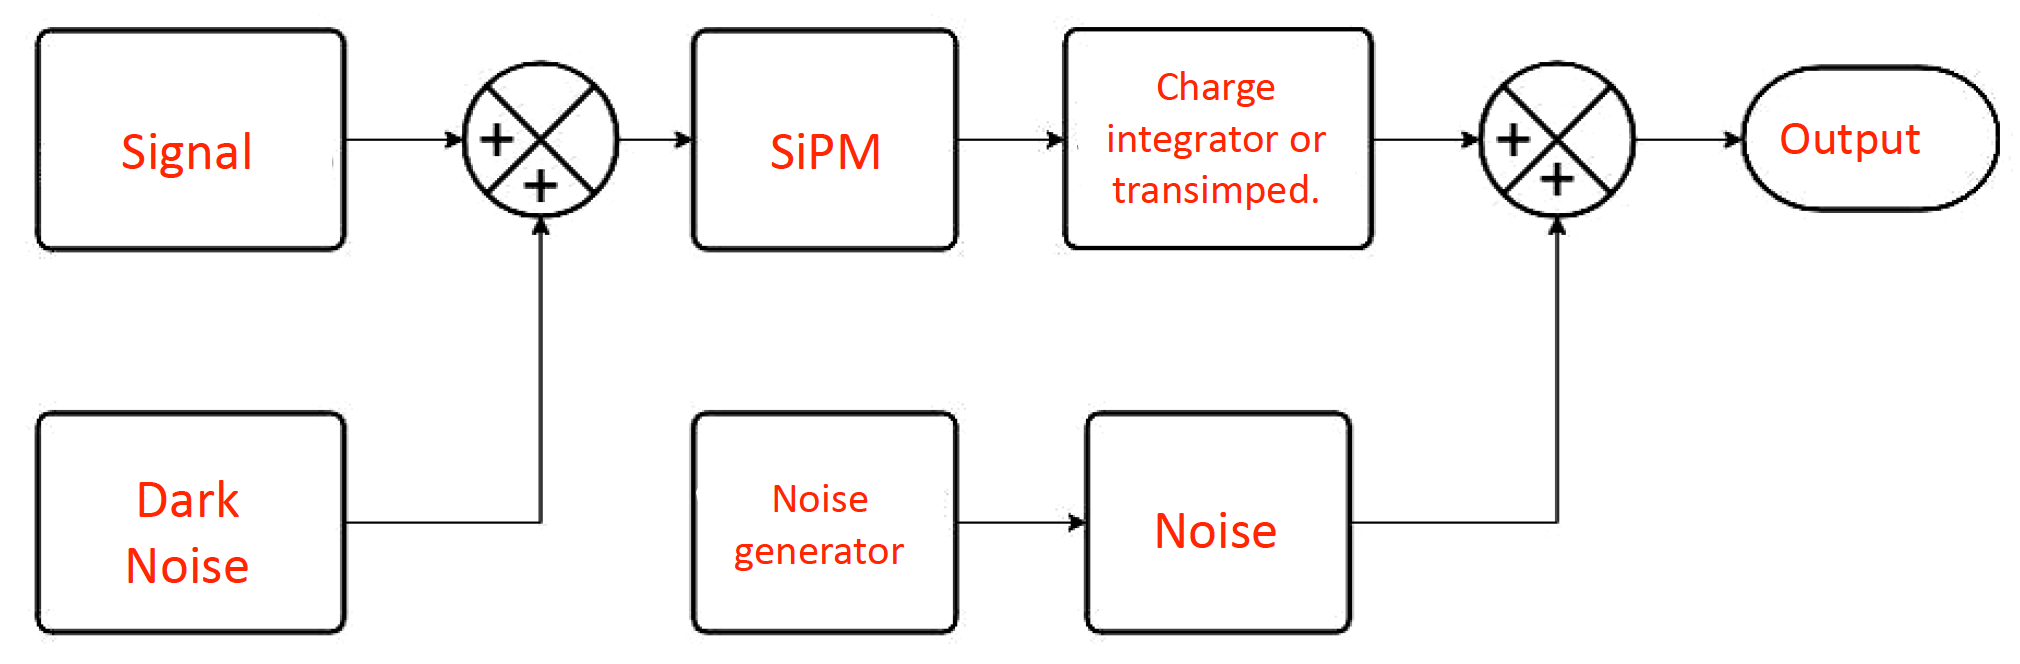
\includegraphics[angle=0,width=8.4cm,height=4cm]{graphics/pds-gang-jorge-2.png}
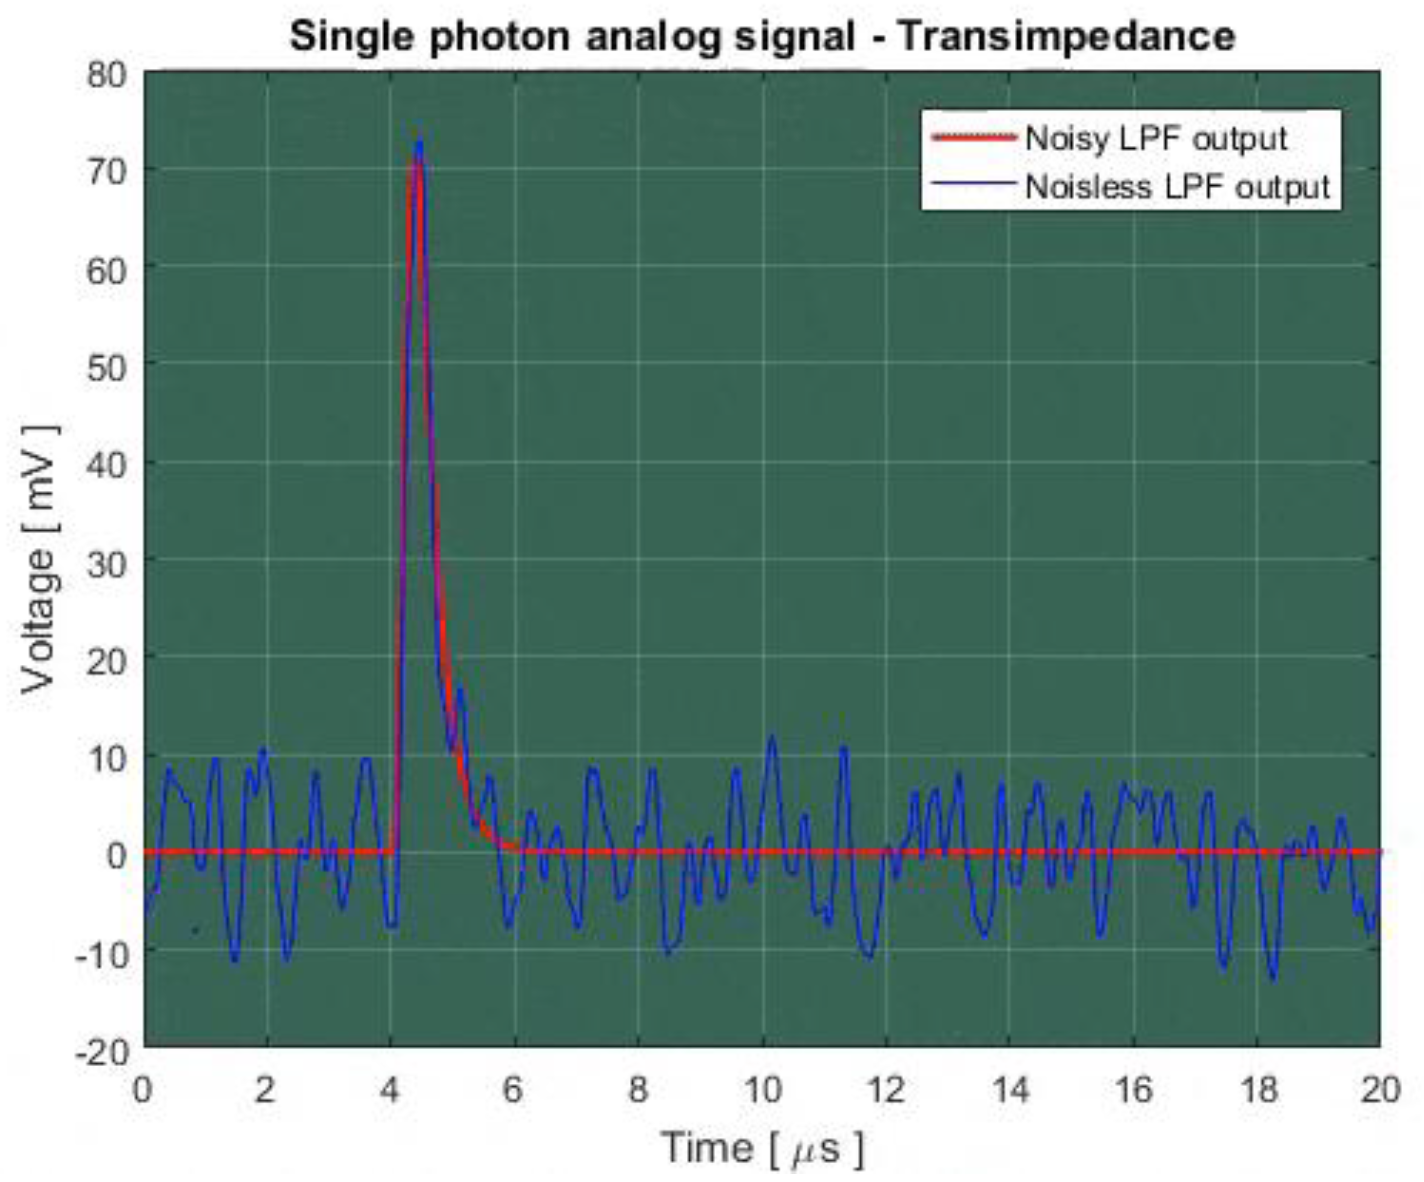
\includegraphics[height=4cm]{graphics/pds-gang-jorge-3.png}
\end{dunefigure}

\begin{dunefigure}[Active ganging circuit to be used in the ICEBERG test stand.]
 {fig:fig-pds-gang-jorge-2}
 {Active ganging circuit to be used in the ICEBERG test stand.}
%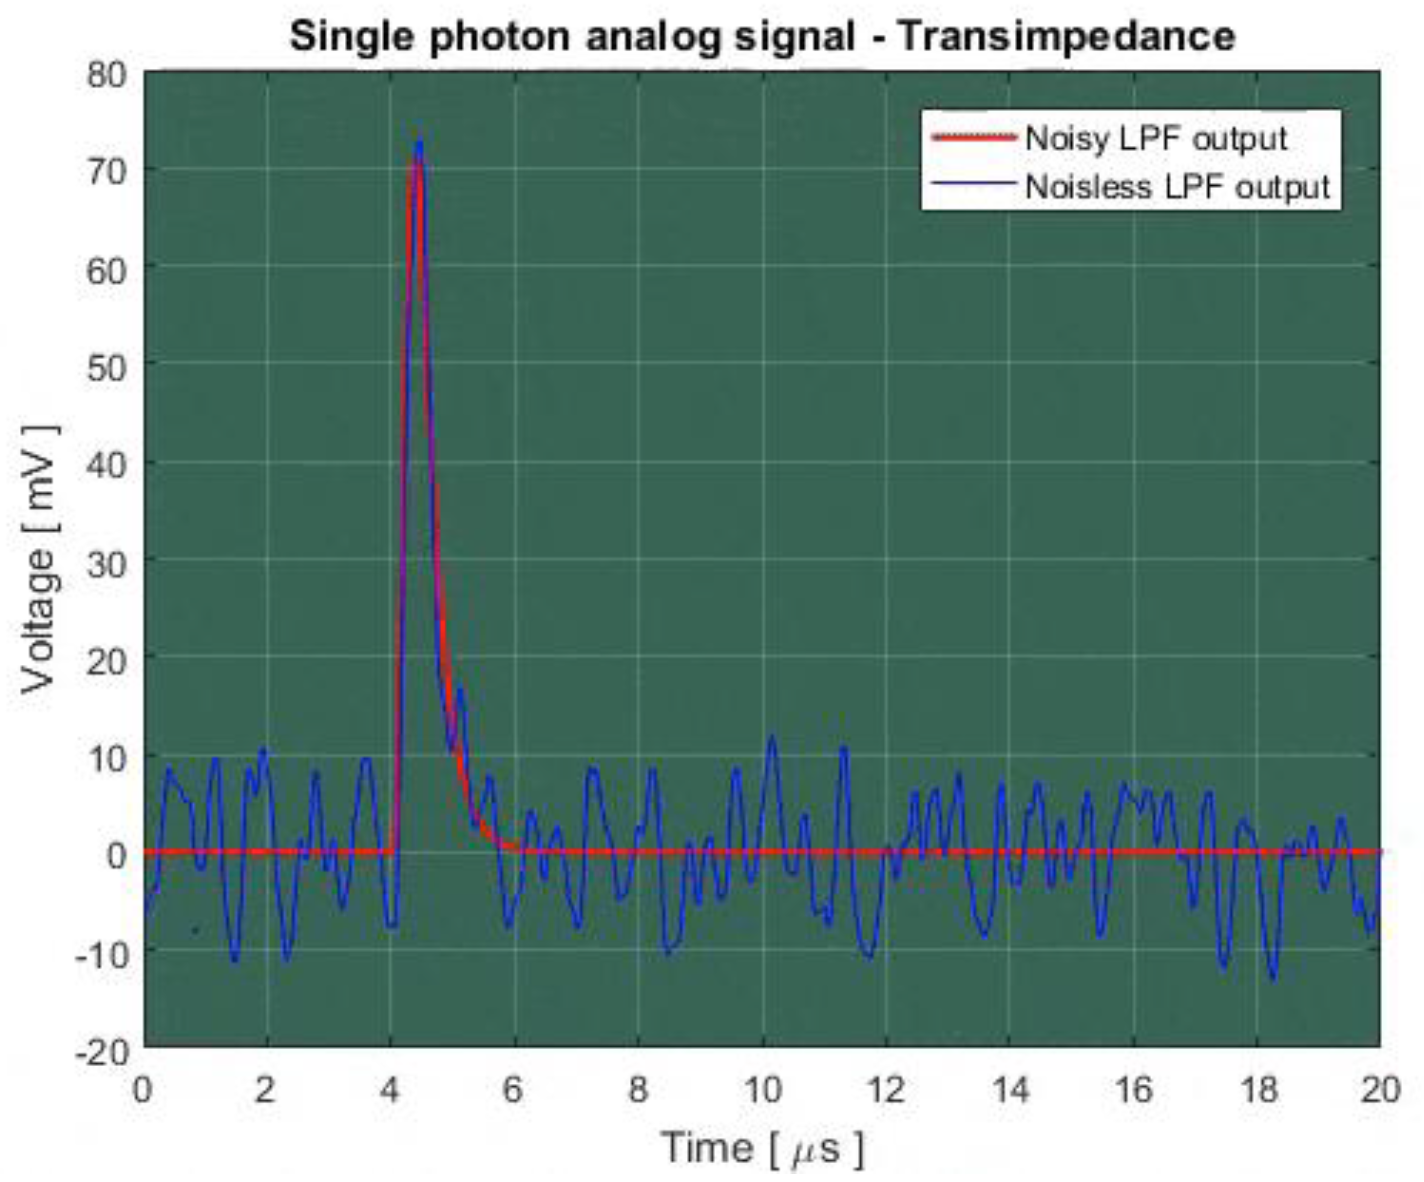
\includegraphics[angle=0,width=8.4cm,height=6cm]{graphics/pds-gang-jorge-3.png}
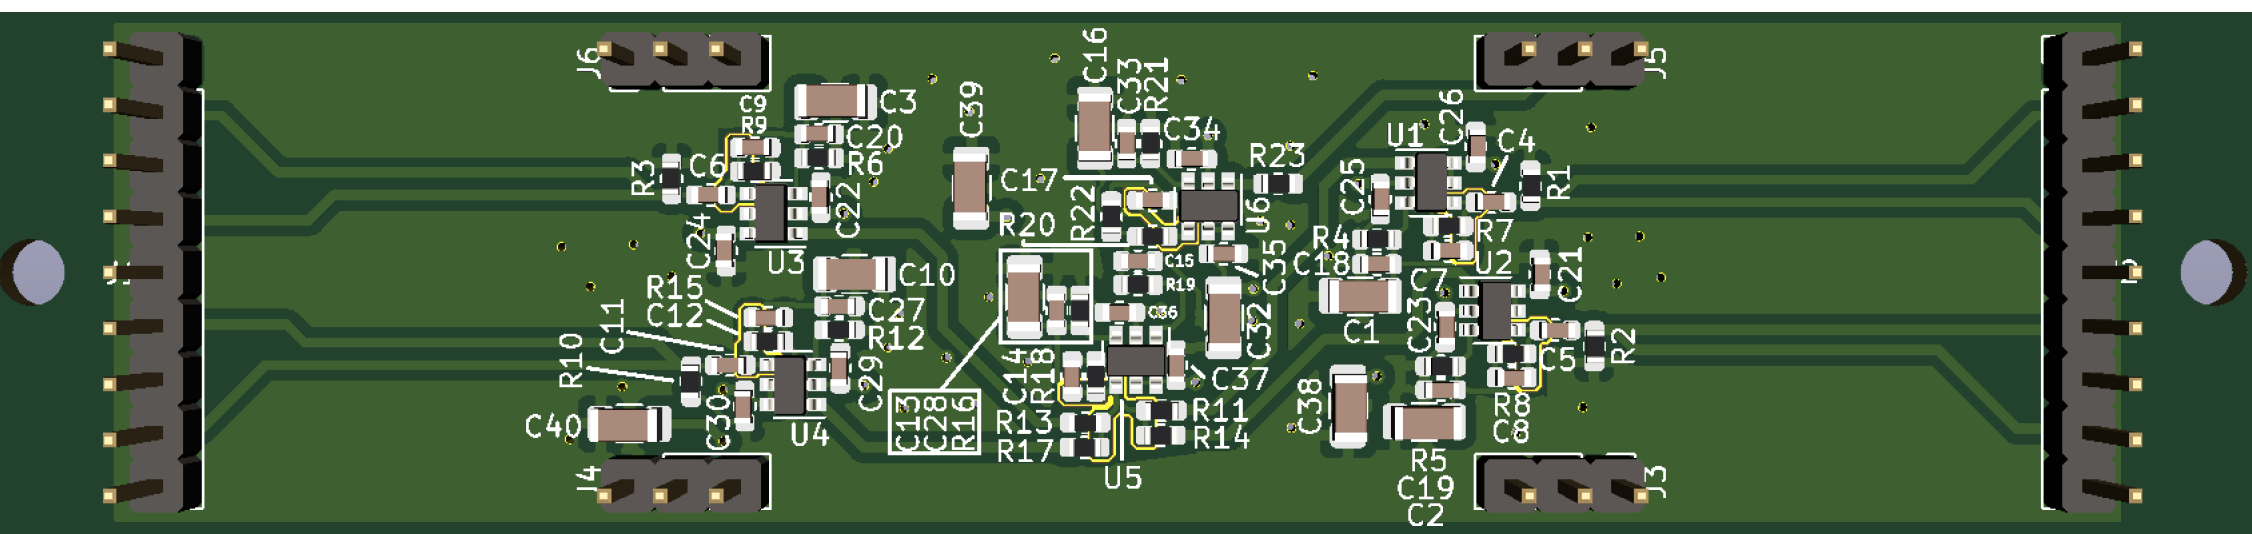
\includegraphics[angle=0,width=8.4cm,height=4cm]{graphics/pds-gang-jorge-4.png}
\end{dunefigure}

The development framework presented above presents a very powerful tool in the design of the electronics. It shows that is possible to gang 48 \dwords{sipm} and distinguish single photon signals with less than 1 $\mu$s width.
%.For single photons there is no significant difference between both models in duration of the pulse and S/N ratio. Preliminary simulations indicates that for 10 photons we don’t see any difference either.
The \dword{s/n} ratio obtained is about \SI{8}{dB}, with all noise effects, including thermal and dark noise contributions.

%\{add more in validation section?}
%5.The optimal sampling rate obtained is >≈ 20 MSPS.
%6.The design of the board for the ICEBERG test stand is ready and in process of fabrication. It includes both designs in the same board, that can be easily exchanged.

%This solution is now used as the baseline summing option for DUNE Far Detector.
%next steps?:This board will also measure the photoelectron collection efficiency when the \dwords{sipm} are coated with \dword{tpb} as a reference for ARAPUCA measurements with a similar ganging level (the summing  board is the same size as the \dword{pdsp} ARAPUCA backplane to facilitate the comparisons). 

%Charge processing requires a charge preamplifier ideally located within the cold environment, so the design must take into consideration the failure risks and the power dissipated into the environment.

%{rjw 11/23/2018: Here should be a description of the Gustavo's and Paraguay groups ganging scheme options (results are in the validation section) - can we identify the FNAL scheme as baseline for the purpose of the TDR draft? Perhaps in the section add the circuit design and drawing of the ganging circuit board that could go in a 10kt production module.}
%{Zelimir added ganging from Gustavo, and from Jorge base on Jorge's 30\% review slides.}

%Typically, arrival time and total charge are the key parameters to be obtained from a detector. Extraction of these parameters 
%is possible using analog or digital systems. Charge preamplifiers will be connected to the output of the detector to integrate current producing a charge proportional output. 

% => this to next steps: In both systems, performance parameters related  to sampling rate, number of bits, power requirements, signal to noise ratio, and interface requirements should be evaluated to arrive to selected solution.  
%Pulse shapes can be fully analyzed to improve detection of a new physics but it will have an important impact on the digitalization frequency.

%**********************************************************************************


%%%%%%%%%%%%%%%%%%%%%%%%%%%%%%%%%%%%%%%%%%%%%%%%%%%%%%%%%%%%%%%%
\subsection{Front-end Electronics Baseline Design}
\label{sec:electronics}
%\{11/28/18  Josh S. text/figures on Mu2e}

Following the successful design, fabrication, operation and performance of \dfirst{ssp} readout in \dword{pdsp}, and with initial high-quality beam and cosmic ray day data collected by the \dword{pdsp} photon system, we are
further cost-optimizing the readout electronics.  To this end we have adopted a lower-cost solution based on lower sampling rate commercial ultrasound ASIC chips rather than digitizers based on flash \dwords{adc}. Inspiration for this cost-effective front-end comes from the system developed for the Mu2e experiment cosmic ray tagger readout system.
Both systems are currently used in the photon detector validation process summarized in Section~\ref{sec:fdsp-pd-validation} to allow direct comparison.


\subsubsection{Front-end Board and Controller}

The readout and digitization of the signals from the active summing board described in Section~\ref{sec:pds-design-ganging} will rely on a set of front-end board (\dword{feb}) readout electronics boards and controller boards, originally designed for the Mu2e experiment~\cite{bib:mu2e_tdr}
at Fermilab. As discussed in Section~\ref{sec:pds-valid-ganging}, preliminary results indicate that the active-summing board and Mu2e electronics \dword{feb} combination will perform well together and, in general, meet the readout requirements for the experiment. The 64~channel \dword{feb} design carried over from Mu2e can be seen in Figure~\ref{fig:feb}. The board has a number of notable features, discussed below. Most importantly, %however, 
the board is designed to utilize commercial, off-the-shelf parts only, and is therefore quite inexpensive compared to other designs. In particular, for the digitization it uses the low-noise, high-gain, and high-dynamic-range commercial \dwords{adc} used in ultrasonic transducers. 

The \dword{feb} is the centerpiece of the baseline readout electronics system.  
The current 64~channel\footnote{This text assumes 64 channels/\dword{feb} when presenting the \dword{feb} and controller. However, we envision 40~channels/\dword{feb} in the final design, corresponding to a single \dword{apa} as described in the ``Next Steps" section.} \dword{feb} relies on commercial ultrasound chips\footnote{Texas Instruments\texttrademark{} 12~bit, 80~MS/s; AFE5807.},
%fixme{check if "next steps" section still there after rearrangement}  
with programmable anti-alias filters and gain stages, to read out the \dword{mppc} signals from the active ganging boards inside the \dword{pd} modules. The board currently takes HDMI inputs, with four channels per input.  Each of the eight ultrasound chips on an \dword{feb} handles eight channels (\SI{120}{mW} per channel) of data using a low-noise preamplifier, a programmable gain amplifier, and a programmable low-pass filter. The information is buffered with a total of \SI{1}{GB} DDR SDRAM, divided in four places, and a set of Spartan~6\texttrademark \dwords{fpga} are used for parallelizing the serial \dword{adc} data, zero suppression, and timing. Each of the four \dwords{fpga} on a board, corresponding to 16 channels, handles two \dword{adc} chips with an available \SI{256}{MB} DDR SDRAM. 

After digitization, the data from each \dword{feb}, in the form of pulses (time-stamp and pulse height) is sent to a master controller via Ethernet, which aggregates the signals from 24 \dword{feb}s, or $64 \times 24=1536$ channels. The 24 \dword{feb}s corresponding to a single controller will come in sets of 12, with each set of 12 \dword{feb}s referenced to a single chassis as shown in %. A picture and schematic of the controller is seen in 
Figure~\ref{fig:controller}. A trigger decision (e.g., accelerator timing signal) can be produced and/or received by the controller and, depending on the decision, each event's digital information is sent to the controller and then to \dword{daq} computers for processing and storage. The controller-to-\dword{daq} connection will rely on a fiber connection, although an Ethernet-based controller output option is available.

% {Since we cannot use this feature (next paragraph) is it worth mentioning? would it need to be removed by the redesigned \dword{feb}? Is that step scheduled?} - remove the follow para

% In addition to its digitization and decision-making abilities, the current \dword{feb} has a number of other notable features. For example, each \dword{feb} contains an onboard Cockcroft-Walton (CW), which is available to generate bias voltage for the \dwords{mppc}. Notably, however, the CW is not currently considered an option for the summing board as it isn't stable enough to bias the differential amplifier. The CW is capable of providing $\approx$+75 V of bias. The board can also apply $\approx$-3~V to the \dword{mppc} anode, allowing the possibility of 78~V. In addition to the \dword{mppc} bias, the \dword{feb}s allow for an on-board current measurement (\SI{100}{pA} resolution) for producing IV curves of \dwords{mppc}. The \dword{feb}s can also be used in stand-alone mode, without a controller, via a telnet interface, which is useful for R\&D purposes and debugging. 
 
\subsubsection{Bandwidth, readout rates, and zero suppression}

\dword{daq} system and data storage limitations impose constraints on the  data flow from the front-end electronics system. 
For example, if it were necessary to read out a \SI{5.5}{\micro\second} waveform (which represents the longest reasonable waveform) 
%is 5.5 mus based on simulation? What happens with overlaping waveforms where longer readout is required, plus calibration etc?
in order to include late-light, the \SI{80}{MS/s}, 12 bit \dword{adc} device would produce a 5.3~kbit waveform. For an envisioned dark count (DC) rate of 250~Hz/channel, this corresponds to a data transfer rate of 53~Mbps/\dword{apa} (1~\dword{apa}=40 channels) or 6.6~MB/s \dword{feb}-to-controller DC rate. This rate approaches the crucial bottleneck in the electronics readout system with a maximum rate of 10~MB/s  %\dword{feb}-to-controller rate 
(per \dword{feb}). However, zero-suppression techniques and multi-channel coincidence/threshold requirements at the \dword{feb} firmware level can be used to significantly mitigate this issue, noting that each on-\dword{feb} \dword{fpga} handles 16 channels. 

It will be necessary to fully understand the system requirements such as the suppression factor in terms of parameters like the readout window length and overall trigger rate to guide the final design. 
Firmware and zero-suppression technique development is in progress and will be informed by the physics and calibration requirements of the \dword{pd}. 
In addition to its bandwidth and DC rate readout capabilities, the system can also  manage a highly-coincident event in which a large number (or all) channels fire at once. For example, a ``maximum (unrealistic)" all-detector event featuring 6000~channels firing at once (corresponding to 4~MB) could be handled by the controller's 24-board write speed of 150~MB/s. 

The baseline electronics readout system performance is consistent with the \dword{daq} interface specification of 8~Gbps per connection, given that  
each \dword{feb} signal corresponds to a maximum of 10~Mbps (240~Mbps total).  

\subsubsection{Power, grounding, and rack schemes} 

Figure~\ref{fig:grounding_power} shows the grounding, power, and data link schemes for the system. The \dword{feb}s are powered via power-over-Ethernet (600 mA, 48 V supply) from the controller. One Cat-6 cable from the controller to each \dword{feb} handles the signal and power simultaneously. The reference planes of the controller and \dword{feb} are isolated on both sides. The grounding scheme calls for each set of 12 \dword{feb}s referenced to a single chassis, with each chassis and corresponding controller on detector ground and the \dword{daq}, connected to each controller via fiber, on building ground. 
 
The rack space and power consumption required by the system assume
a total of 6000 channels with 40 channels/\dword{feb}. This system requires 13 chassis (12 \dword{feb}/chassis) at 6u each and seven controllers (controlling 24 \dword{feb} each) at 1u each. Assuming 42u per rack and with this requirement of $\approx$85u, just over  two racks are needed. The power supply on a controller is 700~W, with each \dword{feb} taking 20~W. 
 

\begin{dunefigure}[64-channel \dword{pds} front-end board (80~MS/s, 12 bit)(left).]
 {fig:feb}
 {A picture of the 64-channel \dword{pds} front-end board (80~MS/s, 12 bit)(left); schematic of the front-end board (right).}
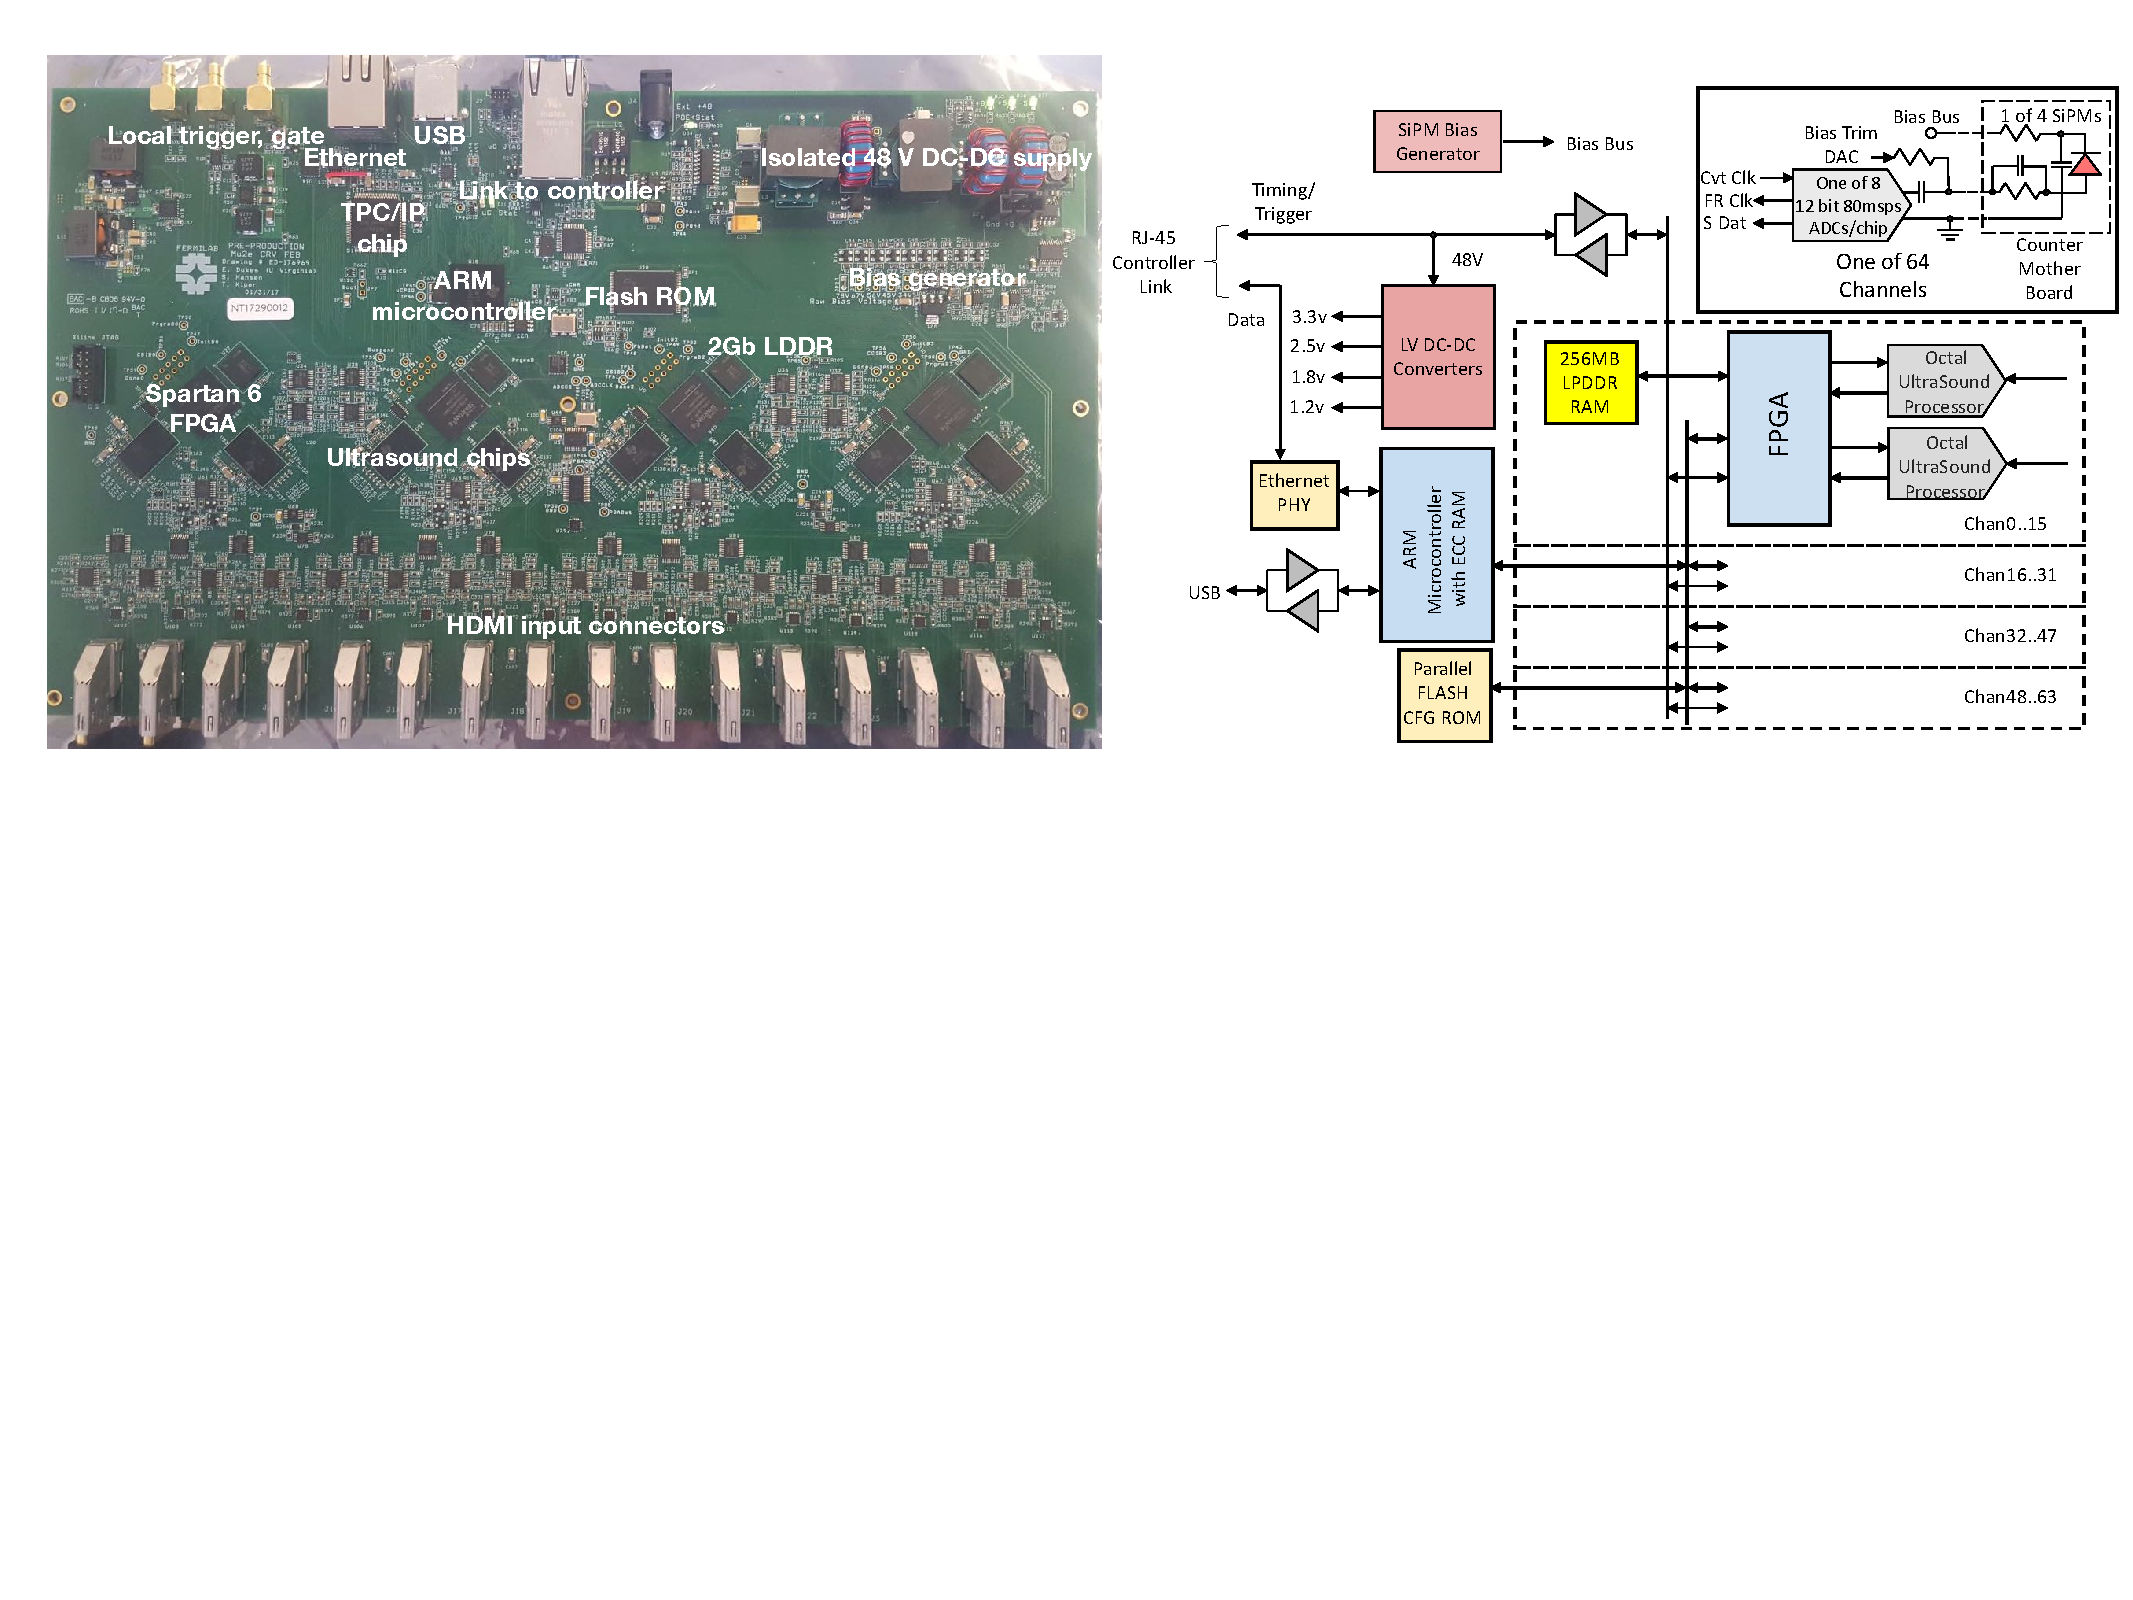
\includegraphics[height=4.8in]{graphics/pds-feb-tdr.pdf} 
\vspace{-6.3cm}
\end{dunefigure}

\begin{dunefigure}[\dword{pds} front-end electronics controller module.]
 {fig:controller}
 {The front (left-bottom) and back views of the controller module (left-top), which is capable of accepting signals from 24 \dword{feb}s; schematic of the controller (right).}
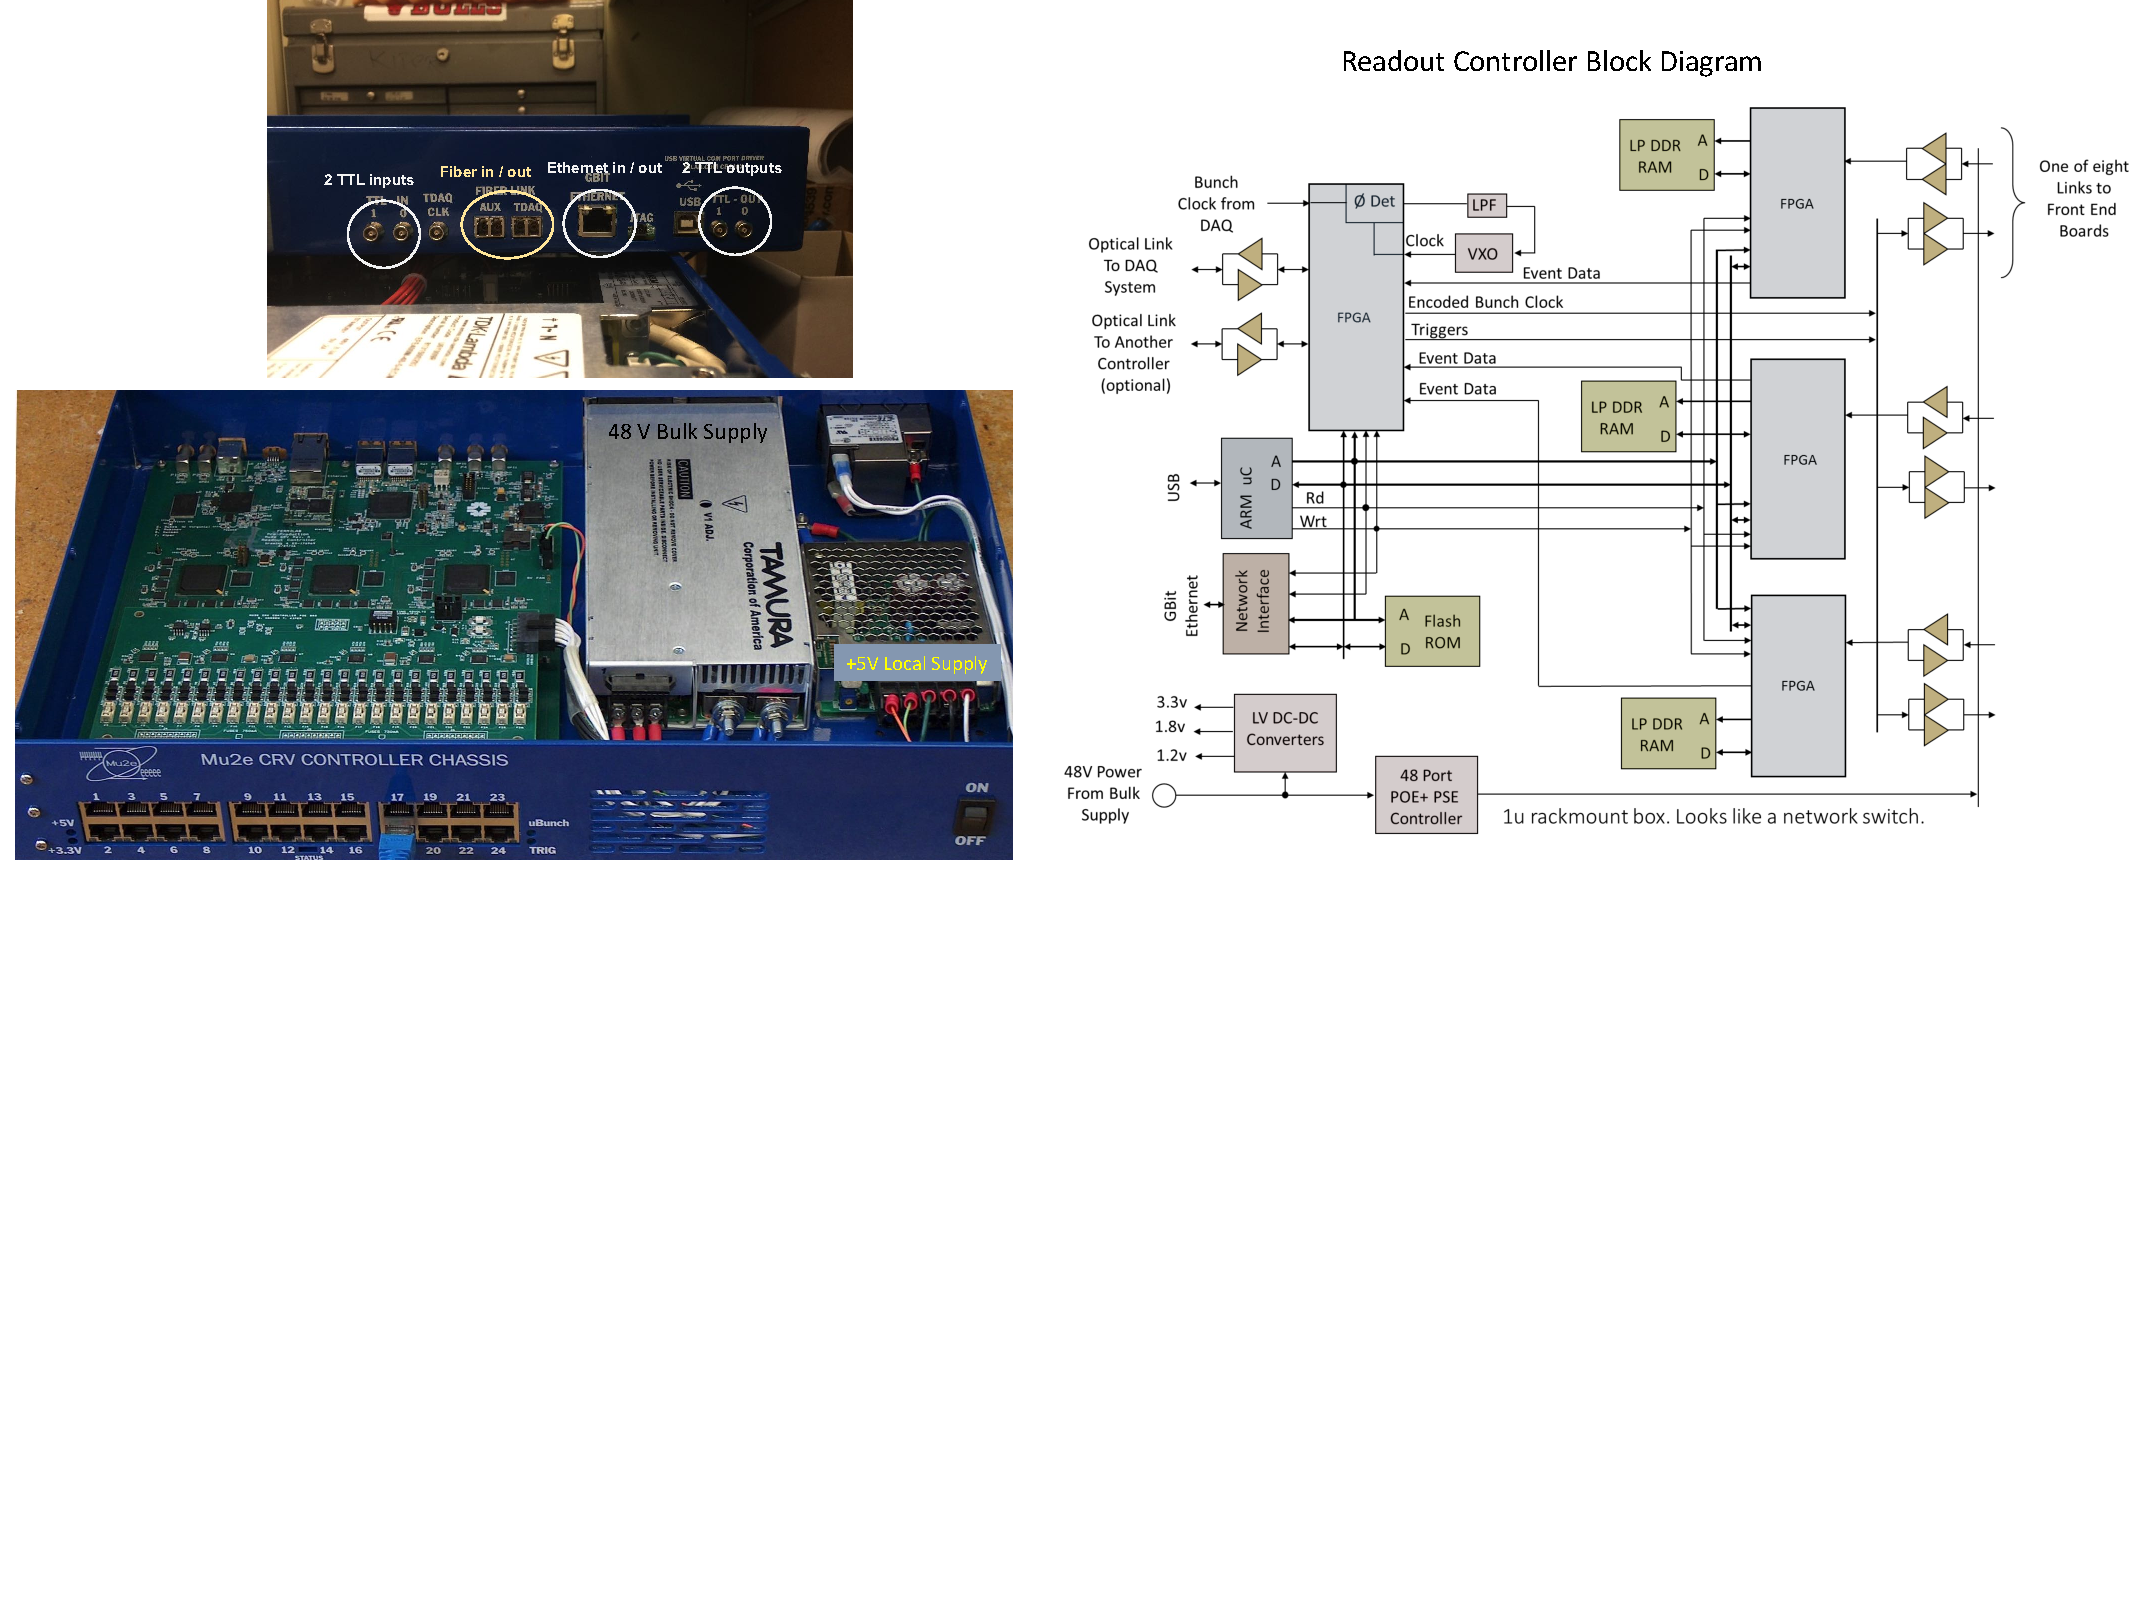
\includegraphics[height=4.8in]{graphics/pds-controller.pdf} 
\vspace{-5.5cm}
\end{dunefigure}

\begin{dunefigure}[\dword{pds} front-end electronics grounding scheme.]
 {fig:grounding_power}
 {Grounding scheme with 1 chassis, containing 12 \dword{feb}s, a controller module, and a \dword{daq} PAC, as an example (left); power and data link arrangement of the \dword{feb} and controller (right).}
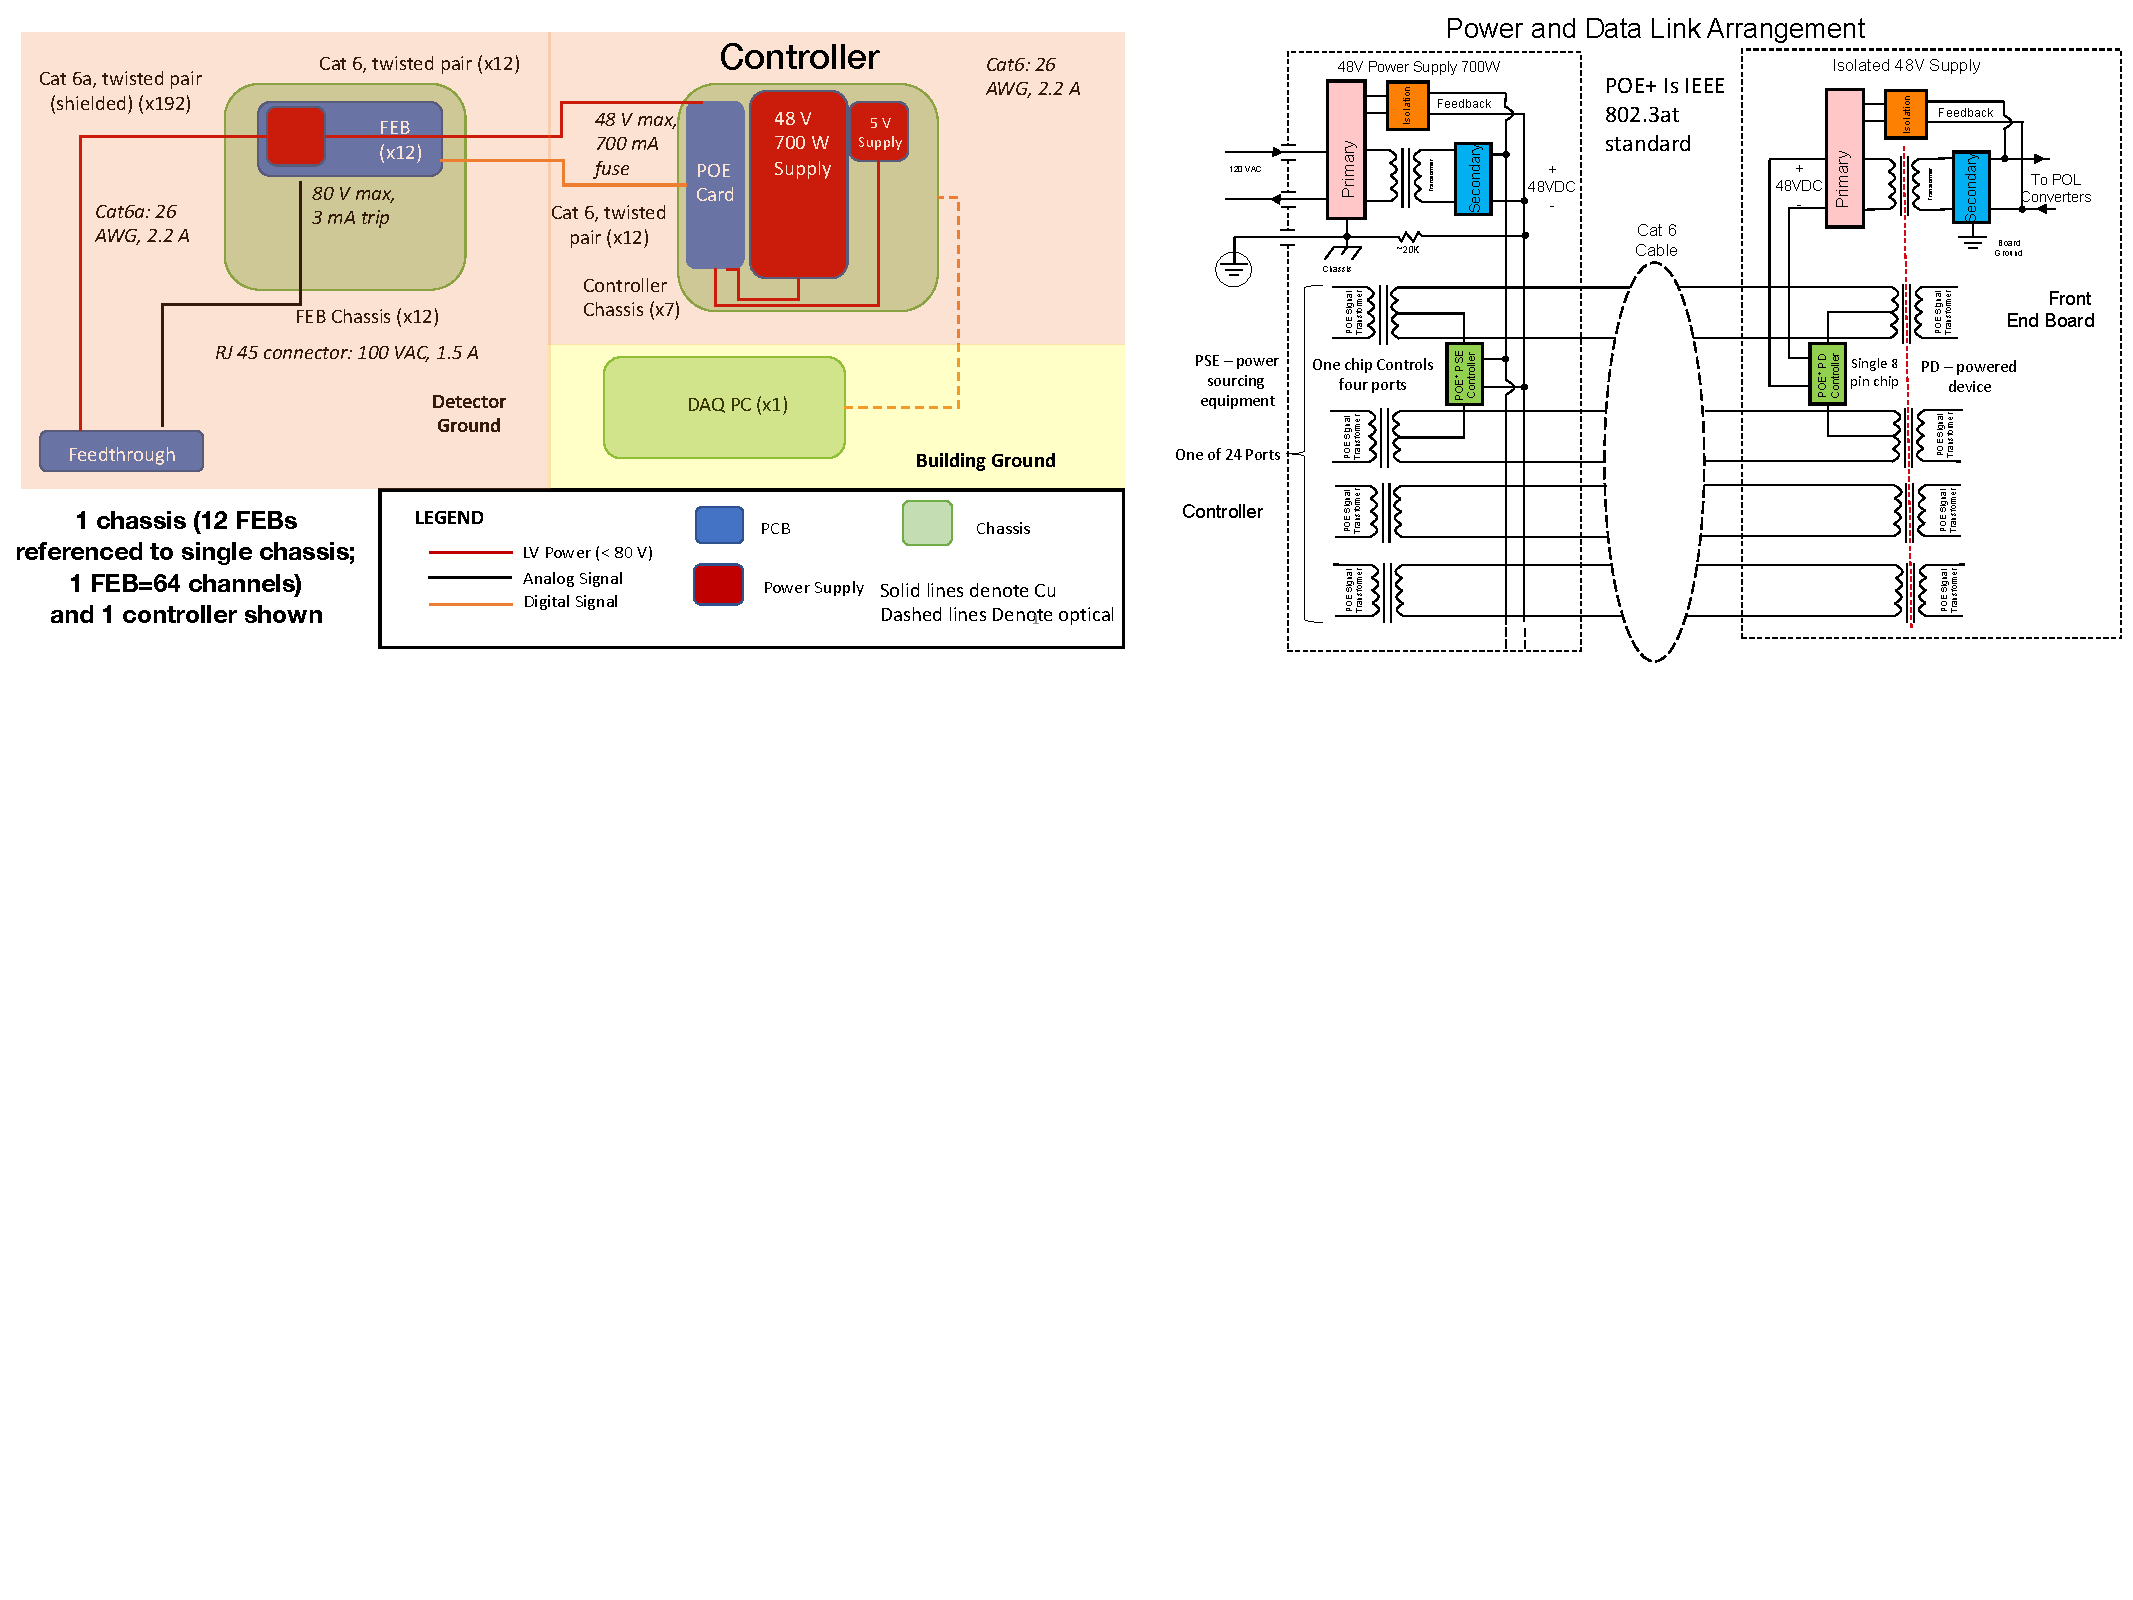
\includegraphics[height=4.8in]{graphics/pds-grounding-power.pdf} 
\vspace{-7.1cm}
\end{dunefigure}


%\begin{figure}[h]
%\begin{centering}
%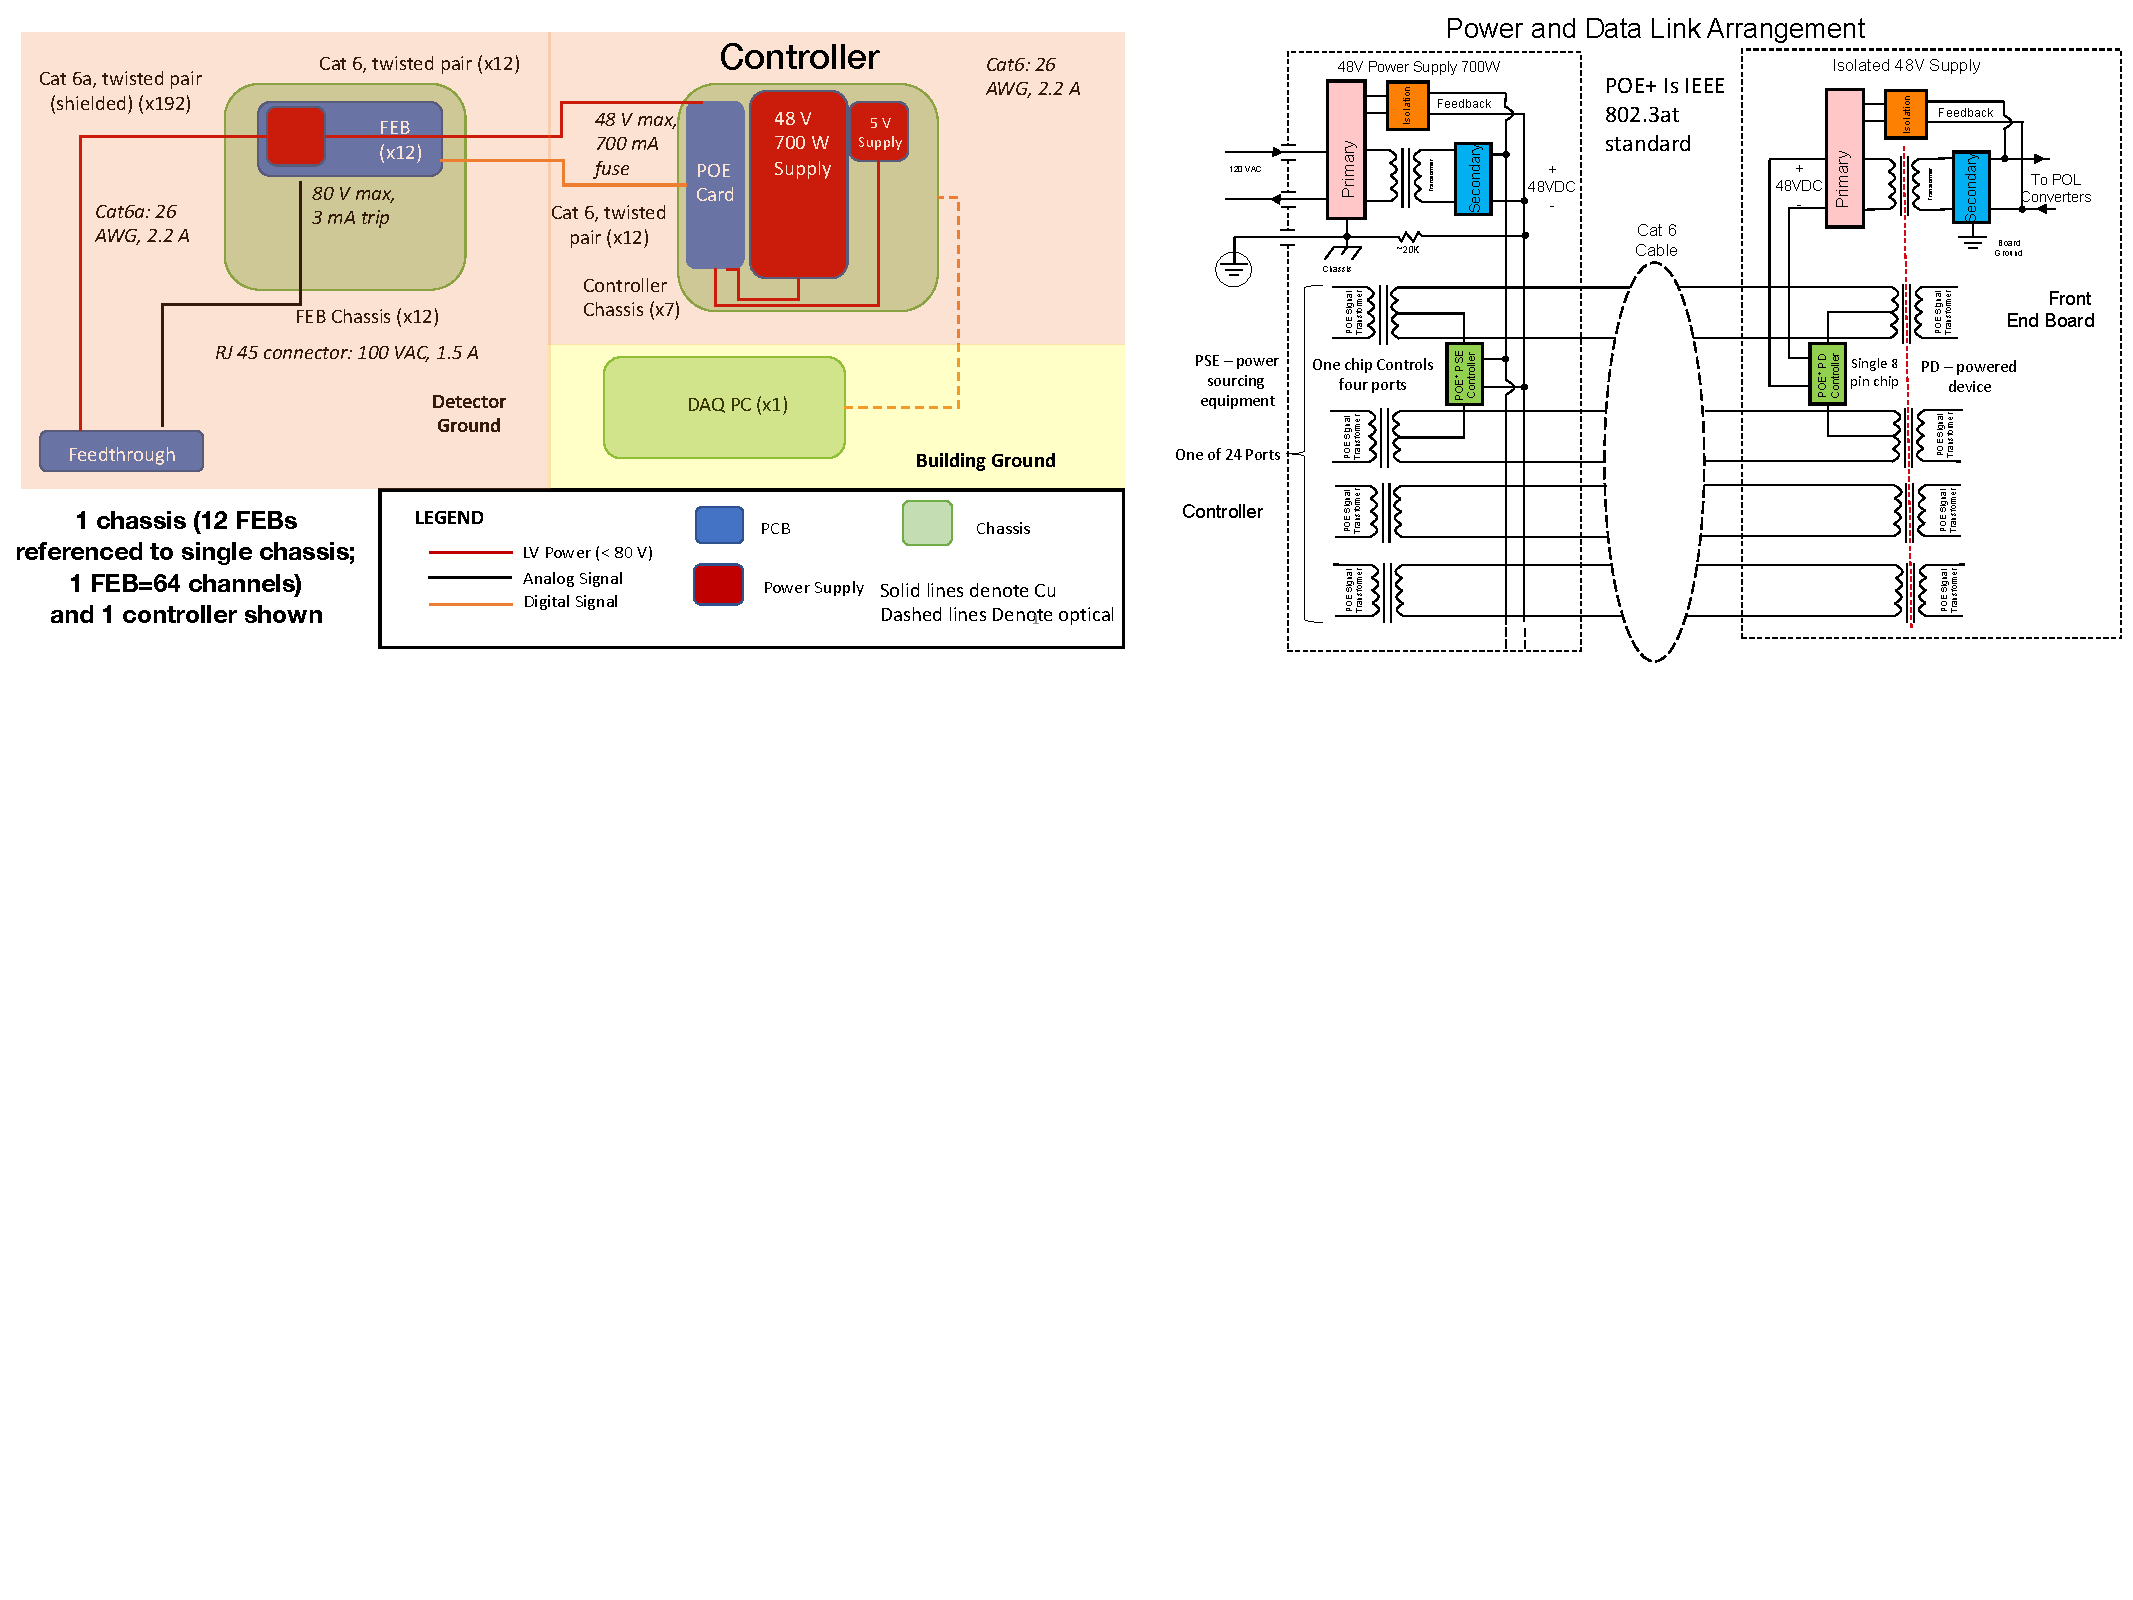
\includegraphics[height=4.8in]{graphics/pds-grounding-power.pdf} 
%\vspace{-7.1cm}
%\caption{(Left) The envisioned grounding scheme with 1 chassis, containing 12 \dword{feb}s, a controller module, and a \dword{daq} PAC, as an example. The power and data link arrangement of the \dword{feb} and controller.}
%\label{fig:grounding_power}
%\end{centering}
%\end{figure}
%%%%%%%%%%%%%%%%%%%%%%%%%%%%%%%%%%%%%%%%%%%%%%%%%%%%%%%%%%%%%%%%%%%%%%%

\subsection{Electronics Next Steps}

%{Zelimir moved sections around 11/29/2018, and also made a pass through the text below.}
%{updated by Toups 11/28/2018}

%Toups start - 11/28/2018
Although the \dword{feb}s developed for the Mu2e cosmic ray veto and proposed here for use in DUNE have %been 
demonstrated the capacity to read out an array of \dwords{mppc} with an adequate \dword{s/n} ratio to provide sensitivity to single photons, there are a number of optimization and development tasks that are being pursued:  
\begin{enumerate}
\item The warm readout electronics presented here assume that only 48 out of the 64 channels on the Mu2e \dword{feb} are populated to better match the 40 ProtoDUNE channels per \dword{apa}.  A prototype board will %be produced to 
test this configuration and validate the associated cost model.  
\item The Mu2e warm readout electronics use last-generation (Xilinx\texttrademark{} Spartan-6) \dwords{fpga} and other components that have since been superceded by newer devices.  Design and prototyping work will %be done to 
incorporate newer \dwords{fpga} (Xilinx Spartan-7 or Artix-7) into the electronics, %which will 
improving their performance and maintainability over the lifetime of the DUNE experiment. The Artix-7 \dwords{fpga} have been implemented with \dword{ssp} readout system used in \dword{pdsp} and therefore the expertise with these system components has been established. 
\item Results from the ICEBERG test stand can determine whether there are sufficient logic resources in the \dwords{fpga} to meet a broad range of possible \dword{daq} requirements expected from the warm readout electronics. To that end the low-cost front-end solution will be compared to existing 14-bit, 150 MS/s \dword{ssp} readout. At present, straightforward zero suppression schemes that can be implemented on the Mu2e board with the current Spartan-6 \dword{fpga} will be tested with respect to potential \dword{daq} data rate limitations.  However, increases in the number of logic cells can be accommodated by switching to more capable but still pinout-compatible devices within the same Xilinx \dword{fpga} family as discussed above.  
\item It may be desirable to increase the dynamic range of the \dwords{adc} used on the \dword{feb}s in order to achieve desired physics goals related to the energy resolution of beam neutrino events.  To this end, %work should be done 
we plan to investigate replacing the TI AFE5807 ultrasound chip with the TI AFE5808 ultrasound chip, which is pinout-compatible but incorporates a 14-bit \dword{adc}.  Ultimately, a prototype board will %need to be built 
incorporate all of the optimizations and improvements listed above.
\end{enumerate}
%Toups end - 11/28/2018
%Although the requirements for the electronics system are not all fully established, it not expected that the system requires novel high-risk techniques and can be developed and fabricated well within the schedule for the \dword{pds}.
The final requirements for the system will be informed by analysis of the data from the readout system implemented in \dword{pdsp} and subsequently data from ICEBERG expected in spring 2019.




%%%%%%%%%%%%%%%%%%%%%%%%%%%%%%%%%%%%%%%%%%%%%%%%%
\section{Calibration and Monitoring}
\label{sec:fdsp-pd-CandM}

The \dword{pds} will incorporate a  pulsed UV-light monitoring and calibration system %described 
to verify the \dword{pd} gain, linearity, and timing resolution, and to monitor stability and the system response over time.  Figure~\ref{fig:pds_calmon_fig1} shows a cartoon of it's  placement in the TPC. This system will also be an important detector commissioning tool before closing the cryostat  
in the cool-down phase, and during the \lar fill.
%- to test the photon detectors, to generate test conditions for low-energy physics, and to 
%make use of it for quick reliable test of PDS when a change in configuration is made.
%	=> Don?t have to wait for cosmic muon coverage of entire detector
Other complementary calibration systems, such as radioactive sources, are described in the \dword{tdr} calibration chapter (Chapter~7). 

\fixme{need a figure showing the design elements}

\begin{dunefigure}[\dword{pdsp} \dword{pd} calibration and monitoring system.]
 {fig:pds_calmon_fig1}
 {Schematic of the \dword{pdsp} \dword{pd} calibration and monitoring system.}
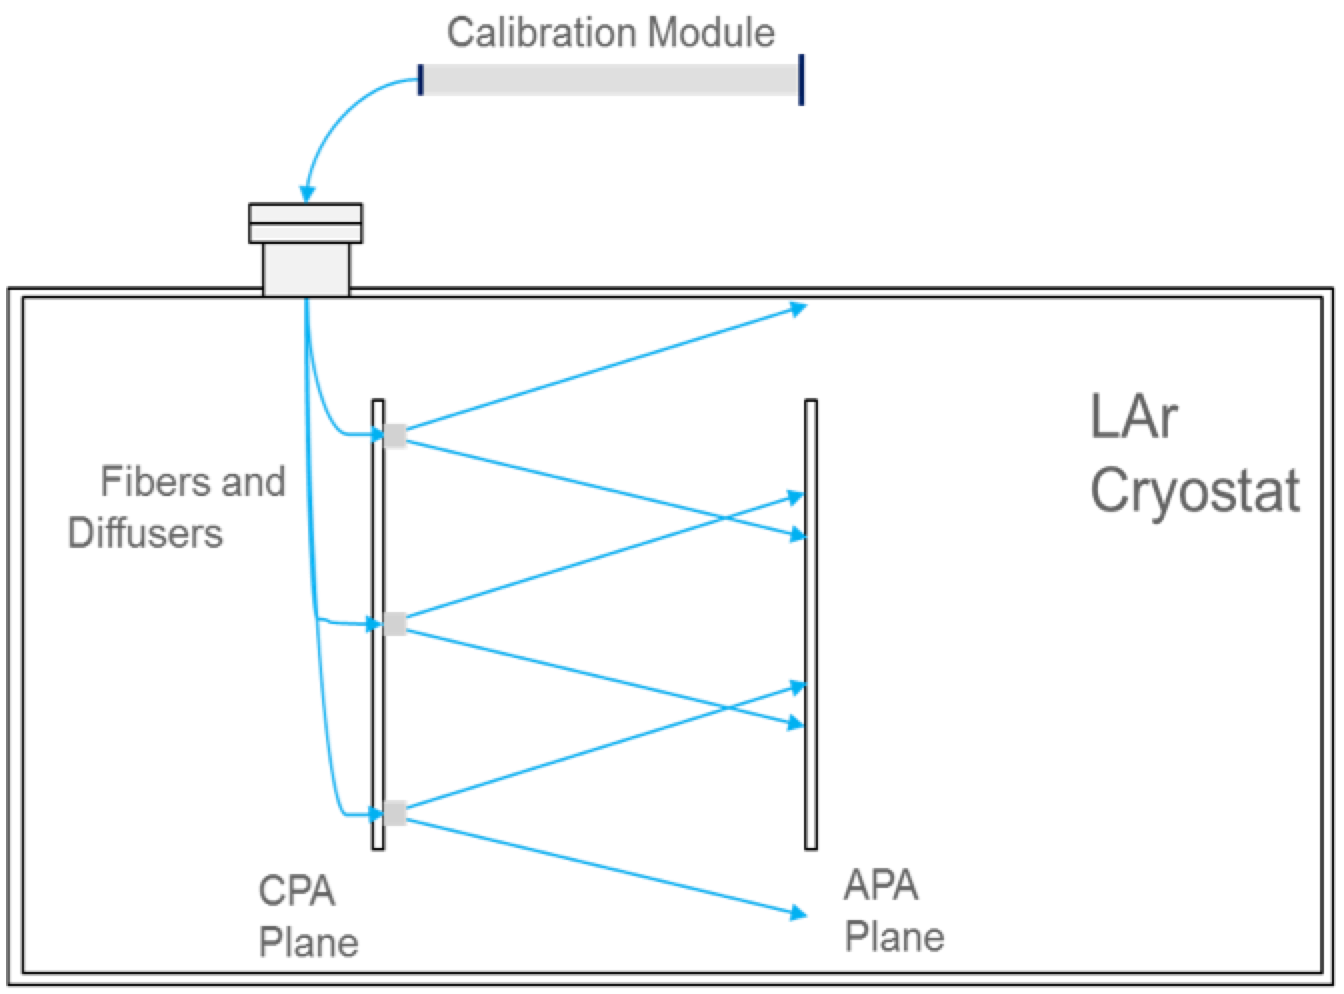
\includegraphics[angle=0,width=8.4cm,height=6cm]{graphics/pds-calmon-fig1-old.png}
\end{dunefigure}

The system hardware consists of both warm and cold components. Diffusers mounted on the \dwords{cpa} provide light sources illuminating \dwords{pd} embedded in the \dword{apa}s. These light diffusers uniformly illuminate the \dword{apa} area containing the \dword{pds} light collection modules. %Cold components (diffusers and fibers) interface with \dword{hv} systems design. 
 Diffusers are installed on the \dwords{cpa} and therefore reside at the %same \dword{cpa} 
 \dword{cpa} potential and interface with \dword{hv} system. 
Quartz fibers are insulators used to transport light from optical feedthroughs (at the cryostat top) through \dword{fc} \dword{gp}, and through \dword{fc} strips to the \dword{cpa} top frame. These fibers are then optically connected to diffusers located on the \dword{cpa} panels. 
The \hv system places a requirement on the fiber electrical resistance to 
protect the cathode from shorting out. 
Warm components include controlled pulsed-UV source (\SIrange{245}{280}{nm}) and warm optics. These warm components will interface with
% \fixme{what's CTF?}
\dword{cisc} and \dword{daq} subsystems. The optical feedthrough is a part of the cryostat interface.
%describe Cali Module. Describe what calibrations could be done

The system has no active components in the liquid argon volume.
The only active component consists of a 1U rack mount
\dword{lcm} sitting outside the cryostat. The \dword{lcm} generates light pulses that propagate through a quartz fiber-optic cable to diffusers at the \dword{cpa} planes to distribute the light uniformly across the \dwords{pd} mounted on the \dword{apa}s.
The \dword{lcm} utilizes the logic and timing control developed to meet DUNE \dword{daq} requirements. It consists of an \dword{fpga}-based control logic unit coupled to an internal LED \dword{lpm} and an additional bulk power supply. The \dword{lpm} uses multiple digital outputs from the control board to control the \dword{lpm} pulse
amplitude, multiplicity, repetition rates, and duration. The unit relies on dedicated \dwords{dac} used to control the \dword{lpm} pulse amplitude. Internal \dword{adc} channels read out a reference photodiode used for pulse-by-pulse monitoring of the LED light output. 
The output of the monitoring diode is available for normalizing the response of the \dwords{sipm} in the detector to the monitoring pulse.

Hardware components will be designed and fabricated based on expertise gained with the \dword{pdsp} prototype system described in Section~\ref{sec:fdsp-pd-validation-candm}.



%\section{PDS Summary Table} 
%\label{sec:pds-config-summary}
% 1/19 Removed summary table from here, it's now up in Scope section. Anne

